\chapter{Dispositif expérimental et méthodes d’analyse}
\label{chap:disp.exp}
\minitoc

%\section{Présentation de l’expérience}
%\section*{Introduction}
%
%\section{Refroidissement}
%
%\section{Imagerie}
%\subsection{Prubleme d'iamgerie et idée numerique}
%
%\section{Confinement transverse}
%
%\section{Confinement longitudinale}
%
%\subsection{Evolution logitudinale}
%
%\section{Outil de sélection spatial}
%
%\subsection{Mesure de distribution de rapidités locales $\rho(x , \theta ) $  pour des systèmes en équilibre}
%
%%\subsection{Piégeage transverses et longitudinale}
%%\section{Outil de sélection spatial}
%%%\section{Mesure de $\rho(x , \theta ) $ }
%
%%\section{Mesure de distribution de rapidités locales $\rho(x , \theta ) $  pour des systèmes en équilibre}

\section*{Introduction}

%\begin{itemize}
%	\item Objectif du chapitre : présentation synthétique de l’expérience
%	\item Distinction claire des contributions : mise en place initiale (précédents doctorants), développement (travail de Léa Dubois), contribution personnelle (prise de données, analyses spécifiques, participation à certaines manipulations)
%	\item Rôle de l’expérience dans l’étude de la dynamique des gaz de Bose 1D
%\end{itemize}

Ce chapitre présente l’expérience utilisée pour étudier les gaz unidimensionnels de rubidium ultra-froids. Nous décrivons l’architecture du dispositif, les méthodes d’imagerie et d’analyse, ainsi que les protocoles expérimentaux auxquels j’ai participé. Le développement initial du refroidissement et du piégeage avant la puce a été réalisé par d’anciens doctorants \cite{jacqm2012,Fang2014,Johnson2016} . La mise en place du piégeage sur la puce a été réalisé par d’anciens doctorants \cite{jacqm2012,Fang2014,Johnson2016,schem2019,L.Dubois2024}. La mise en place du système de sélection spatiale à l’aide d’un \gls{DMD}  a été initiée par Léa Dubois \cite{L.Dubois2024}, alors en première année de doctorat à mon arrivée. Mon travail s’est concentré principalement sur la prise de données, l’analyse et la participation à certaines expériences spécifiques telles que l'étude de l’expansion longitudinale et la mesure de la distribution de rapidité locale.



\paragraph{Objectif du chapitre}  
Ce chapitre a pour objectif de fournir une présentation synthétique et structurée du dispositif expérimental utilisé pour étudier la dynamique de gaz de Bose unidimensionnels ultra-froids. Il constitue un socle indispensable pour comprendre les protocoles expérimentaux développés au cours de ma thèse et les analyses présentées dans les chapitres suivants.

\paragraph{Architecture générale}  
Nous présentons d'abord l’architecture complète de l’expérience, depuis la production des atomes jusqu’à leur imagerie, en passant par les étapes de refroidissement, de piégeage magnétique sur puce, de manipulation optique, et de génération de potentiels. Cette description s’accompagne d’une mise en contexte des contributions historiques au dispositif.

\paragraph{Contributions successives et personnelles}  
Une attention particulière est portée à la répartition chronologique des contributions. Les étapes initiales (source atomique, \gls{PMO}, piège \acrshort{DC} pour \acrlong{DC} en anglais) ont été développées par d’anciens doctorants. La mise en place du piégeage 1D sur puce ainsi que l’utilisation du \gls{DMD} pour la sélection spatiale ont été réalisées au cours de la thèse de L. Dubois \cite{L.Dubois2024}. Mon travail s’inscrit dans cette continuité et concerne principalement la prise de données, l’analyse de protocoles dynamiques, ainsi que la participation à certaines opérations de maintenance et d’optimisation du système.

\paragraph{Rôle du dispositif dans la thèse}  
Ce dispositif permet d’explorer des phénomènes hors équilibre dans des gaz quantiques 1D. Il constitue une plateforme particulièrement adaptée à l’étude de protocoles d’expansion, de sondes locales, ou de dynamiques guidées par \gls{GHD}, qui sont au cœur de cette thèse.




%\section{Présentation générale de l’expérience}
%\subsection{Vue d’ensemble du dispositif}
%\begin{itemize}
%    \item Architecture générale : production, piégeage, manipulation et imagerie.
%    \item Systèmes étudiés : gaz de rubidium 87 dans des pièges 1D.
%    \item Objectifs : exploration de dynamiques hors équilibre.
%\end{itemize}
%
%\subsection{Historique et contributions successives}
%\begin{itemize}
%    \item Étapes de refroidissement et piégeage initial : travaux antérieurs (voir thèses citées).
%    \item Développement du piégeage 1D sur puce et du DMD : thèse de Léa Dubois.
%    \item Contributions personnelles : prise de données, protocoles dynamiques, analyse.
%\end{itemize}

\section{Le dispositif expérimental}
\subsection{Système laser et contrôle de fréquence}
\label{sec:systeme_laser}

%\paragraph{Laser maître 1 : référence de fréquence}
%La référence principale de fréquence pour l'ensemble des faisceaux utilisés dans l'expérience est fournie par un laser à cavité étendue, développé au SYRTE. Ce laser est asservi par spectroscopie d’absorption saturée sur la transition D2 du $^{87}$Rb, au croisement des transitions $|F=2\rangle \rightarrow |F'=2,3\rangle$. Ce signal de référence est utilisé pour verrouiller les autres sources laser par battement optique.

\paragraph{Laser maître 1 : référence de fréquence}
La stabilité en fréquence de l’ensemble des faisceaux employés dans l’expérience est assurée par un laser à cavité étendue conçu selon un schéma du \gls{SYRTE}. Ce laser est verrouillé par spectroscopie d’absorption saturée sur la raie D2 du $^{87}$Rb, en ciblant le croisement des transitions $|F=2\rangle \rightarrow |F'=2,3\rangle$. Ce verrouillage fournit la référence absolue de fréquence à partir de laquelle les autres sources laser sont synchronisées par battement optique.

%\paragraph{Laser repompeur}
%Un laser DFB (Distributed Feedback Diode) est utilisé pour produire le faisceau repompeur, permettant de transférer les atomes retombés dans l’état $|F=1\rangle$ vers l’état $|F=2\rangle$. Ce laser est asservi à une fréquence distante de 6\,GHz de celle du maître 1, en utilisant un montage de battement optique et mélange avec un oscillateur à 6.6\,GHz. Une diode Fabry-Perot injectée par la DFB permet d’amplifier la puissance au-delà de 100\,mW.
%
%\paragraph{Laser repompeur}
%Le faisceau de repompage, qui permet de transférer les atomes piégés dans l’état $|F=1\rangle$ vers l’état $|F=2\rangle$, est généré par une diode DFB (Distributed Feedback). Sa fréquence est décalée de 6,GHz par rapport au maître 1 grâce à un système de battement optique combiné à un mélange avec un oscillateur micro-onde à 6.6,GHz. Une diode Fabry–Perot, injectée par la DFB, permet d’augmenter la puissance de sortie au-delà de 100,mW.

\paragraph{Laser repompeur}
Le faisceau de repompage, qui transfère les atomes tombé  dans l’état $|F=1\rangle$ vers l’état $|F=2\rangle$, est produit par une diode \gls{DFB} . Sa fréquence est décalée de $6~GHz$ par rapport au maître 1 par battement optique et mélange avec un oscillateur à micro-ondes de $6.6~GHz$. Une diode Fabry–Perot, injectée par la \gls{DFB}, élève la puissance de sortie au-delà de $200~mW$.

%\paragraph{Laser maître 2 : laser principal de manipulation}
%Un second laser à cavité étendue, identique au maître 1, est asservi par battement optique à la fréquence du maître 1. Il est amplifié par un amplificateur à semi-conducteur évasé (Tapered Amplifier), permettant d’atteindre une puissance de sortie supérieure à 1\,W. Ce faisceau est ensuite divisé en plusieurs branches pour alimenter :
%\begin{itemize}
%    \item le Piège Magnéto-Optique (PMO),
%    \item la mélasse optique,
%    \item le pompage optique,
%    \item l’imagerie par absorption,
%    \item le faisceau de sélection.
%\end{itemize}

\paragraph{Laser maître 2 : source principale de manipulation}
Un second laser à cavité étendue, est verrouillé par battement optique sur la fréquence du maître 1. L’émission est amplifiée au moyen d’un amplificateur à semi-conducteur évasé (\gls{TA}), fournissant plus de $1\,W$ en sortie. Le faisceau ainsi produit est distribué vers différentes parties de l’installation expérimentale : alimentation du piège magnéto-optique \gls{PMO}, formation de la mélasse optique, réalisation du pompage optique, imagerie par absorption,génération du faisceau de sélection.


%\paragraph{Contrôle de fréquence et polarisation}
%Les fréquences des différents faisceaux sont ajustées via des Modulateurs Acousto-Optiques (AOM), tandis que leur polarisation et leur intensité sont contrôlées à l’aide de cubes PBS en combinaison avec des lames demi-onde motorisées ou fixes. Cette configuration assure une grande flexibilité dans la mise en œuvre des différentes phases expérimentales.

\paragraph{Gestion des fréquences et polarisations}
%Les ajustements de fréquence des divers faisceaux sont réalisés à l’aide de modulateurs acousto-optiques (AOM).
Les faisceaux peuvent être interrompus soit à l’aide d’obturateurs mécaniques, soit via des modulateurs acousto-optiques (en anglais \gls{AOM}). Ces derniers offrent un temps de commutation beaucoup plus court que les systèmes mécaniques, car ils permettent de sélectionner uniquement un ordre de diffraction non nul et d’éteindre en quelque $ms$ le faisceau en interrompant l’alimentation radiofréquence. L’intensité et la polarisation sont réglées via des cubes séparateurs (\gls{PBS}) associés à des lames demi-onde, fixes ou motorisées. Ce dispositif offre une grande souplesse pour adapter la configuration optique aux différentes étapes de l’expérience.

%\paragraph{Remarque}
%Une description plus détaillée du montage laser et de son verrouillage peut être trouvée dans la thèse de A.~Johnson~\cite{Johnson2016}. L’ensemble a été maintenu et utilisé sans modifications majeures au cours de ma thèse.

\paragraph{Note}
Une présentation plus exhaustive du montage laser et de son système de verrouillage est disponible dans la thèse de A.Johnson\cite{Johnson2016}. Le dispositif a été conservé dans son architecture d’origine tout au long de mes travaux, avec seulement un entretien régulier.


\subsection{Production et refroidissement des atomes}
%{\color{blue}
%\begin{itemize}
%    \item Source chaude de rubidium, MOT, molasses optique.
%    \item Refroidissement à des températures sub-$\mu~K$ Refroidissement sub-Doppler (détails renvoyés aux travaux précédents).
%\end{itemize}
%}
%Le dispositif expérimental permet de produire des gaz de rubidium ultra-froids, avec pour objectif final l’obtention de gaz unidimensionnels dans le régime quantique dégénéré. La production suit une séquence expérimentale déjà bien établie, initialement développée par d’anciens doctorants (voir par exemple la thèse d’A. Johnson~\cite{Johnson2016}), puis réoptimisée au début de la thèse de Léa-Dubois ~\cite{L.Dubois2024} sous la supervision d’I. Bouchoule.

Le dispositif expérimental permet de produire des gaz ultra-froids de rubidium, en vue d’obtenir des gaz unidimensionnels dans le régime quantique dégénéré. La séquence expérimentale suit un protocole établi, initialement développé par d’anciens doctorants (voir par exemple la thèse d’A. Johnson~\cite{Johnson2016}) et réoptimisé au début de la thèse de L. Dubois~\cite{L.Dubois2024} sous la supervision d’I. Bouchoule.

%\paragraph{Libération des atomes de rubidium}
%Les atomes de $^{87}$Rb sont libérés à partir d’un \emph{dispenser}, placé directement dans l’enceinte à vide, sur le côté de la monture de la puce atomique. Ce composant, parcouru par un courant de \( 4.5\,\mathrm{A} \) pendant environ \( 5\,\mathrm{s} \), émet un flux d’atomes thermiques dans la chambre à vide.

\paragraph{Libération des atomes de rubidium}
Les atomes de $^{87}$Rb sont émis à partir d’un dispositif appelé \emph{dispenser}, placé directement dans l’enceinte à vide à proximité de la monture de la puce atomique. Un courant de \( 4.5\,\mathrm{A} \) y est appliqué pendant environ \( 5\,\mathrm{s} \), ce qui génère un flux d’atomes thermiques dans la chambre à vide.

\paragraph{Capture par le piège magnéto-optique (\gls{PMO})}
Les atomes thermiques sont ralentis et confinés dans un piège magnéto-optique. Quatre faisceaux laser (dont deux réfléchis par la puce) combinés à un champ quadrupolaire magnétique produit par des bobines permettent de former un nuage atomique situé à quelques millimètres de la surface de la puce.


\paragraph{Rapprochement vers la puce}
Le nuage est rapproché de la surface de la puce en transférant le champ quadrupolaire des bobines vers un champ homogène produit par ces bobines, combiné au champ généré par le fil en forme de U de la puce (fil bleu, Fig.~\ref{fig:puce}). Le courant dans ce fil est ajusté lentement de \(3.6\,\mathrm{A}\) à \(1.5\,\mathrm{A}\), ce qui positionne le nuage à quelques centaines de micromètres de la surface.

\paragraph{Mélasse optique}
Après la capture dans le \gls{PMO}, une étape de mélasse optique est appliquée pour refroidir davantage le nuage atomique, au-delà de la limite de Doppler. La mélasse optique repose sur l’utilisation de faisceaux laser légèrement désaccordés en fréquence par rapport à la résonance de la transition atomique utilisée pour le refroidissement et polarisés de manière appropriée, qui interagissent avec les atomes selon le mécanisme de refroidissement sub-Doppler.

Le principe physique est le suivant : les atomes en mouvement voient les faisceaux laser avec un décalage Doppler, ce qui modifie la probabilité d’absorption selon leur vitesse et leur position. Combiné avec les effets de polarisation (notamment les forces de type Sisyphus dans un champ de polarisation variable), cela crée un potentiel de friction optique qui ralentit les atomes. Contrairement au refroidissement Doppler standard, la mélasse optique permet de réduire l’énergie cinétique des atomes en dessous de la limite Doppler, atteignant des températures beaucoup plus basses.

Ainsi, cette étape permet d’obtenir un nuage plus dense et plus froid, condition essentielle pour les manipulations ultérieures et la formation de gaz unidimensionnels dans le régime quantique dégénéré.

\paragraph{Pompage optique}
Enfin, les atomes sont préparés dans l’état magnétique \( |F=2,\,m_F=2\rangle \) par pompage optique. Un faisceau circulairement polarisé \( \sigma^+ \), résonant sur la transition \( |F=2\rangle \rightarrow |F'=2\rangle \), assure la polarisation du nuage (Fig~\ref{chap:5:fig:hiperfin}).


\begin{figure}[H]
	\centering
	\begin{tikzpicture}
			\begin{scope}[shift={(2,0)}]
				%\begin{scope}[transform canvas={scale=1.6}]
				\begin{scope}[scale=1.0]
					
% Définition des couleurs avec les codes HTML
\definecolor{colorOne}{HTML}{443E46}
%\definecolor{colorTwo}{HTML}{F6DEB8}
\definecolor{colorTwo}{HTML}{FFFFFF}

\definecolor{colorThree}{HTML}{908CA4}
\definecolor{colorFour}{HTML}{57659E}
\definecolor{colorFive}{HTML}{C57284}
\definecolor{colorSix}{HTML}{FF5B69}

% Raccourcis pour les couleurs
\def\colorOne{colorOne}
\def\colorTwo{colorTwo}
\def\colorThree{colorThree}
\def\colorFour{colorFour}
\def\colorFive{colorFive}
\def\colorSix{colorSix}

\definecolor{colorGold}{HTML}{FFD700}
\def\colorGold{colorGold}



\begin{scope}

	
	%Base L ,S 
	\draw[]
	
		(-1,0) edge [ thick,line width=0.5ex, color = \colorOne ] node [shift={(0cm,-0mm)}, pos = 0.5 , above  ]{{ \color{\colorOne}$5S$}} (1 , 0) 
		
	;
	
	
	% 5S1/2 Fine 	
	\begin{scope}[shift={(1cm,0cm)}]
		\draw
			(0,0) edge [dashed ,line width=0.45ex, color = \colorOne ] (1 , 0)
		;
		
		\begin{scope}[shift={(1cm,0cm)}]
			\draw[shift={(0cm,0cm)}]
				(0,0) edge [ thick,line width=0.5ex, color = \colorOne ] node [shift={(0cm,-1mm)}, pos = 0.75 , above ]{{ \color{\colorOne}$ 5S_{1/2}$}} (2 , 0)
			;
			
			\draw
				(0.25,0.01) edge [decoration={
   							markings,
    						mark connection node=midnode,
    						mark=at position 0.5 with {
      							\node[draw = none ,fill= white ,transform shape , opacity = 1] (midnode) {{\color{\colorFive} \fontsize{8pt}{8pt}\selectfont
					$D_1 : 795~nm$}};
    							}
 						 	},
  							postaction={decorate}, thick, line width=0.5ex, <->, >=Stealth, color=colorFive ] 
   				(0.25,4.29)		
   				(0.75,0.01) edge[decoration={
   							markings,
    						mark connection node=midnode,
    						mark=at position 0.4 with {
      							\node[draw = none ,fill= white ,transform shape , opacity = 1] (midnode) {{\color{\colorFour}\fontsize{8pt}{8pt}\selectfont $D_2 : 780~nm$}};
    							}
 						 	},
  							postaction={decorate}, thick, line width=0.5ex, <->, >=Stealth, color=colorFour ]
   				(0.75,5.74)	
				;
			
			%Hyperfine
			\begin{scope}[shift={(2cm,0cm)}]
				\draw	
					(0,0) edge [dashed ,line width=0.45ex, color = \colorOne ] (1 , 0.75)
					(0,0) edge [dashed ,line width=0.45ex, color = \colorOne ] (1 , -0.75)
				;
				
				\draw[shift={(1cm,0mm)}]
					(0,0.75) edge [ thick,line width=0.5ex, color = \colorOne ] node [shift={(0cm,0mm)}, pos = 1 , right ]{{ \color{\colorOne}$ F = 2 $}} (2 , 0.75)
					(0,-0.75) edge [ thick,line width=0.5ex, color = \colorOne ] node [shift={(0cm,0mm)} , pos = 1 , right ]{{ \color{\colorOne}$ F = 1$}} (2 , -0.75)
				;
				
				
			\end{scope}
		\end{scope}
	\end{scope}
	
	
	% 5P1/2 3/2 Fine 
	\begin{scope}[shift={(1cm,5cm)}]
		
		\draw[shift={(-2cm,0cm)}]
			(0,0) edge [ thick,line width=0.5ex, color = \colorOne ] node [shift={(0cm,-0mm)}, pos = 0.5 , above ]{{ \color{\colorOne}$5P$}} (2 , 0)
		;

		\draw
			(0,0) edge [dashed ,line width=0.45ex, color = \colorOne ] (1 , 0.75)
			(0,0) edge [dashed ,line width=0.45ex, color = \colorOne ] (1 , -0.75)
		;
		
		%5P1/2 
		\begin{scope}[shift={(1cm,-0.75cm)}]		
			\draw
				(0,0) edge [ thick,line width=0.5ex, color = \colorOne ] node [shift={(0cm,-1mm)} , pos = 0.75 , above  ]{{ \color{\colorOne}$ 5P_{1/2}$}} (2 , 0)
			;		
		\end{scope}
		
		%5P3/2 
		\begin{scope}[shift={(1cm,0.75cm)}]		
			\draw
				(0,0) edge [ thick,line width=0.5ex, color = \colorOne ] node [shift={(0cm,-1mm)} , pos = 0.75 , above  ]{{ \color{\colorOne}$ 5P_{3/2}$}} (2 , 0)
			;
			
			%Hyperfine
			\begin{scope}[shift={(2cm,0cm)}]
				\draw
					(0,0) edge [dashed ,line width=0.45ex, color = \colorOne ] (1 , 2.25)
					(0,0) edge [dashed ,line width=0.45ex, color = \colorOne ] (1 , 0.75)
					(0,0) edge [dashed ,line width=0.45ex, color = \colorOne ] (1 , -0.75)
					(0,0) edge [dashed ,line width=0.45ex, color = \colorOne ] (1 , -2.25)
				;
				
				\draw[shift={(1cm,0mm)}]
					(0,2.25) edge [ thick,line width=0.5ex, color = \colorOne ] node [shift={(0cm,0mm)} , pos = 1 , right ]{{ \color{\colorOne}$ F' = 3$}} (2 , 2.25)
					(0,0.75) edge [ thick,line width=0.5ex, color = \colorOne ] node [shift={(0cm,0mm)}, pos = 1 , right ]{{ \color{\colorOne}$ F' = 2 $}} (2 , 0.75)
					(0,-0.75) edge [ thick,line width=0.5ex, color = \colorOne ] node [shift={(0cm,0mm)} , pos = 1 , right ]{{ \color{\colorOne}$ F' = 1$}} (2 , -0.75)
					(0,-2.25) edge [ thick,line width=0.5ex, color = \colorOne ] node [shift={(0cm,0mm)} , pos = 1 , right ]{{ \color{\colorOne}$ F' = 0$}} (2 , -2.25)
					
					(0.55,1.5) edge [dotted ,line width=0.5ex, color = \colorOne ]  (1.45 , 1.5)
					
					(1.25,1.75) edge [dotted ,line width=0.5ex, color = \colorSix ]  (2.15 , 1.75)
					(1.25,2.75) edge [dotted ,line width=0.5ex, color = \colorSix ]  (2.15 , 2.75)
				;
				
				\draw[shift={(1cm,0mm)}]
					(0.25,0.75) edge [decoration={
   							markings,
    						mark connection node=midnode,
    						mark=at position 0.5 with {
      							\node[draw = none ,fill= white ,transform shape , opacity = 1] (midnode) {{\color{\colorFive} \fontsize{4pt}{8pt}\selectfont$267.2~MHz$}};
    							}
 						 	},
  							postaction={decorate}, thick, line width=0.5ex, <->, >=Stealth, color=colorFive ] 
   					(0.25,2.25)		
				;
			\end{scope}		
		\end{scope}
		
	\end{scope}
	
	\draw[shift={(5cm,0mm)}]	
   		(1.75,-0.75) edge[decoration={
   							markings,
    						mark connection node=midnode,
    						mark=at position 0.5 with {
      							\node[draw = none ,fill= white ,transform shape , opacity = 1] (midnode) {{\color{\colorFive}\fontsize{4pt}{8pt}\selectfont $6.874~GHz$}};
    							}
 						 	},
  							postaction={decorate}, thick, line width=0.5ex, <->, >=Stealth, color=colorFive ]
   		(1.75,0.75)
   		(.25,-0.75) edge[decoration={
   							markings,
    						mark connection node=midnode,
    						mark=at position 0.38 with {
      							\node[draw = none ,fill= white ,transform shape , opacity = 1] (midnode) {{\color{\colorSix}\fontsize{8pt}{8pt}\selectfont Repompeur}};
    							}
 						 	},
  							postaction={decorate}, thick, line width=0.5ex, <->, >=Stealth, color=colorSix ]
   		(.25,6.55)	
   		(1.0,0.75) edge[decoration={
   							markings,
    						mark connection node=midnode,
    						mark=at position 0.2 with {
      							\node[draw = none ,fill= white ,transform shape , opacity = 1] (midnode) {{\color{\colorSix}\fontsize{8pt}{8pt}\selectfont Maitre 1}};
    							}
 						 	},
  							postaction={decorate}, thick, line width=0.5ex, <->, >=Stealth, color=colorSix ]
   		(1.0,7.25)	
   		(1.75,0.75) edge[decoration={
   							markings,
    						mark connection node=midnode,
    						mark=at position 0.18 with {
      							\node[draw = none ,fill= white ,transform shape , opacity = 1] (midnode) {{\color{\colorSix}\fontsize{8pt}{8pt}\selectfont Maitre 2 }};
    							}
 						 	},
  							postaction={decorate}, thick, line width=0.5ex, <->, >=Stealth, color=colorSix ]
   		(1.75,7.75)
		;


\end{scope}
	
			
				\end{scope}
			
				%\draw[color = red , scale = 0.5 , draw = none  ] (-2 , -1) rectangle (5, 6) ; 	
			\end{scope}
					
	\end{tikzpicture}
	\caption{Structure hyperfine (transitions D1 et D2) de l’atome de Rubidium $^{87}$Rb. Les longueurs d’onde des différents lasers utilisés dans l’expérience sont représentées en rouge vif (Fig adaptée de \cite{L.Dubois2024})}
	\label{chap:5:fig:hiperfin}
\end{figure}






\subsection{Piégeage magnétique sur puce}
%{\color{blue}
%\begin{itemize}
%    \item Présentation de la puce atomique.
%    \item Confinement transverse et longitudinal.
%    \item Régime 1D : conditions d’accès (\(\hbar \omega_\perp \gg k_B T\)).
%    \item Problèmes de rugosité, stabilité magnétique.
%\end{itemize}
%}

\begin{figure}[H]
	\centering
	\begin{tikzpicture}
			\begin{scope}[shift={(0,0)}]
				\begin{scope}[transform canvas={scale=0.6}]
				%\begin{scope}[scale=0.5]
					
% Définition des couleurs avec les codes HTML
\definecolor{colorOne}{HTML}{443E46}
%\definecolor{colorTwo}{HTML}{F6DEB8}
\definecolor{colorTwo}{HTML}{FFFFFF}

\definecolor{colorThree}{HTML}{908CA4}
\definecolor{colorFour}{HTML}{57659E}
\definecolor{colorFive}{HTML}{C57284}
\definecolor{colorSix}{HTML}{FF5B69}

% Raccourcis pour les couleurs
\def\colorOne{colorOne}
\def\colorTwo{colorTwo}
\def\colorThree{colorThree}
\def\colorFour{colorFour}
\def\colorFive{colorFive}
\def\colorSix{colorSix}

\definecolor{colorGold}{HTML}{FFD700}
\def\colorGold{colorGold}


\begin{scope}
	%\drawgrid{-6}{6}{0}{10}	;
	\draw
		(-5,0) edge[thick,line width=0.5cm, color = \colorFour] node [pos = 0 , above]{{\color{\colorTwo} $\bm{U}$}} (-5,2.75)
		(-5,2) edge[thick,line width=1.5cm, color = \colorFour] (5,2)
		(5,2.75) edge[thick,line width=0.5cm, color = \colorFour] (5,0)
	;
	\draw[thick,line width=0.5cm, color = \colorSix]
		(-5.5,0) -- node [pos = 0 , above]{{\color{\colorTwo} $\bm{Z}$}}  (-5.5,3.) -- (5.00,3.0) -- (5.00,6.35)
	;
	\draw[shift={(-5.65cm , 3.35cm)} , thick,line width=0.2cm, color = \colorFive]
		(0,3) -- (0,0)-- (2.5,0)-- node [pos = 1 , above]{d}(2.5,3)
	;
	\draw[shift={(2.15cm , 3.35cm)} , thick,line width=0.2cm, color = \colorFive , opacity = 1]
		(0,3) -- node [pos = 0 , above]{d'} (0,0)-- (2.5,0)-- (2.5,3)
	;
	\draw[shift={(-5.4cm , 3.6cm)} , thick,line width=0.3cm, color = \colorThree , opacity = 1]
		(0,2.75) -- (0,0)-- (1.7,0)-- node [pos = 1 , above]{D} (1.7,2.75)
	;
	\draw[shift={(2.7cm , 3.6cm)} , thick,line width=0.3cm, color = \colorThree , opacity = 1]
		(0,2.75) -- node [pos = 0 , above]{D'} (0,0)-- (1.7,0)-- (1.7,2.75)
	;
	
	\draw[shift={(-3.0cm , 3.6cm)} , thick,line width=0.2cm, color = \colorThree , opacity = 1]
		(0.06,2.75) -- (0.06,0.095)-- (4.94,0.095)-- (4.94,2.75)
	;
	
	\draw[shift={(-3.0cm , 3.6cm)} , thick,line width=0.03cm, color = \colorTwo , opacity = 1]
		(-0.035,2.75) -- (-0.035,0)-- (5.035,0)-- (5.035,2.75)
		(0.035,2.75) -- (0.035,0.07)-- (4.965,0.07)-- (4.965,2.75)
		(0.105,2.75) -- (0.105,0.14)-- (4.895,0.14)-- (4.895,2.75)
	;
	
	\draw[shift={(-3.0cm , 4cm)} , thick,line width=0.1cm, color = \colorOne , opacity = 1 , <->]
		(0.0,0.095) -- node[pos = 0.5, above]{$2l = 1390~\mu m$} (5.0,0.095)
		
	;
	
	\draw[shift={(-3.0cm , 5cm)} , thick,line width=0.1cm, color = \colorOne , opacity = 1 , <->]
		(-0.5,0.095) -- node[pos = 0.5, above]{$2L = 1890 \,\mu m$} (5.5,0.095)
	;
	
	\draw[shift={(-6.0cm , -0.25cm)} , thick,line width=0.1cm, color = \colorOne , opacity = 1 ]
		(-0.5,0)edge[, ->] node[pos = 1.01, above]{\fontsize{20pt}{8pt}\selectfont$\bm{\vec{e}_x}$} (12,0)
		(0,-0.5) edge[, ->] node[pos = 0.99, left]{\fontsize{20pt}{8pt}\selectfont$\bm{\vec{e}_u}$} (0,7.25)
	;
	
\end{scope}
	
			
				\end{scope}
			
				\draw[color = red , scale = 0.5 , draw = none  ] (-6 , -1) rectangle (6, 9) ; 
				\node[below , shift={(-3cm , 5cm)}] at (0,0) {\fontsize{15pt}{8pt}\selectfont a)};	
			\end{scope}
			
			\begin{scope}[shift={(9,0)}]
				\begin{scope}[transform canvas={scale=0.6}]
				%\begin{scope}[scale=0.5]
					% Définition des couleurs avec les codes HTML
\definecolor{colorOne}{HTML}{443E46}
%\definecolor{colorTwo}{HTML}{F6DEB8}
\definecolor{colorTwo}{HTML}{FFFFFF}

\definecolor{colorThree}{HTML}{908CA4}
\definecolor{colorFour}{HTML}{57659E}
\definecolor{colorFive}{HTML}{C57284}
\definecolor{colorSix}{HTML}{FF5B69}

% Raccourcis pour les couleurs
\def\colorOne{colorOne}
\def\colorTwo{colorTwo}
\def\colorThree{colorThree}
\def\colorFour{colorFour}
\def\colorFive{colorFive}
\def\colorSix{colorSix}

\definecolor{colorGold}{HTML}{FFD700}
\def\colorGold{colorGold}



\begin{scope}


	\draw[shift={(-2cm , 1.25cm)} , thick,line width=2.5cm, color = \colorThree , opacity = 1 ]
		(0,0) -- node[shift={(-0.75cm , -0.5cm)} , pos = 0.0, right , color = \colorTwo]{{\color{\colorTwo} \fontsize{15pt}{8pt}\selectfont \bf SiC} } (13.5,0)
	;
	\draw[shift={(-2cm , 3.5cm)} , thick,line width=2.cm, color = \colorFour , opacity = 1 ]
		(0,0) -- node[shift={(-0.75cm , -0.5cm)} , pos = 0.0, right , color = \colorTwo]{{\color{\colorTwo} \fontsize{15pt}{8pt}\selectfont \bf BCB} } (13.5,0)
	;
	\draw[shift={(-2cm , 5.cm)} , thick,line width=1.cm, color = \colorGold , opacity = 1 ]
		(0,0) -- node[shift={(-0.2cm , 0.cm)} , pos = 0.0, right , color = \colorTwo]{{\color{\colorOne} \fontsize{15pt}{8pt}\selectfont \bf Au} } (13.5,0)
	;
	
	
	\begin{scope}[shift={(2cm , 2.5cm)}]
		\draw[thick,line width=0.1cm , rounded corners=0cm,  color = \colorTwo , fill = \colorFive ] 
			(0,0) rectangle (1,1)
			;
		% croix
		\draw[ thick,line width=0.1cm , color = \colorOne] 
			(0,0) -- (1,1)
			(0,1) -- (1,0)
		;
		\node[left , shift={(-0.3cm , 0.5cm)} , color = \colorTwo] at (0,0) {{\color{\colorTwo}\fontsize{20pt}{8pt}\selectfont$-I$}};
	\end{scope}
	
	\begin{scope}[shift={(5cm , 2.5cm)}]
		\draw[thick,line width=0.1cm , rounded corners=0cm,  color = \colorTwo , fill = \colorFive ] 
			(0,0) rectangle (1,1)
			;
		% croix
		\fill[ thick,line width=0.1cm , color = \colorOne] 
			(0.5,0.5) circle (0.1cm);
		\node[left , shift={(-0.3cm , 0.5cm)} , color = \colorTwo] at (0,0) {{\color{\colorTwo}\fontsize{20pt}{8pt}\selectfont$I$}};
	\end{scope}
	
	\begin{scope}[shift={(8cm , 2.5cm)}]
		\draw[thick,line width=0.1cm , rounded corners=0cm,  color = \colorTwo , fill = \colorFive ] 
			(0,0) rectangle (1,1)
			;
		% croix
		\draw[ thick,line width=0.1cm , color = \colorOne] 
			(0,0) -- (1,1)
			(0,1) -- (1,0)
		;
		\node[left , shift={(-0.3cm , 0.5cm)} , color = \colorTwo] at (0,0) {{\color{\colorTwo}\fontsize{20pt}{8pt}\selectfont$-I$}};
	\end{scope}
	
	\draw[shift={(2.5cm , 2.cm)}]
		(0,0) edge [decoration={
   							markings,
    						mark connection node=midnode,
    						mark=at position 0.5 with {
      							\node[draw = none ,fill= \colorThree ,transform shape , opacity = 1] (midnode) {{\color{\colorTwo} \fontsize{10pt}{8pt}\selectfont
					$d = 15 \mu m $}};
    							}
 						 	},
  							postaction={decorate},
		thick,line width=0.1cm , <->, color = \colorTwo	, >=Stealth	
		] (3,0)
	;
	
	\draw[shift={(3.8cm , 3.cm)}]
		(0,0) edge [decoration={
   							markings,
    						mark connection node=midnode,
    						mark=at position 0.65 with {
      							\node[draw = none ,fill= \colorGold ,transform shape , opacity = 1] (midnode) {{\color{\colorOne} \fontsize{10pt}{8pt}\selectfont
					$d$}};
    							}
 						 	},
  							postaction={decorate},
		thick,line width=0.1cm , <->, color = \colorOne , >=Stealth	
		] (0,3)
	;
	
	\draw[shift={(10.25cm , 0.cm)}]
		(0,0) edge [decoration={
   							markings,
    						mark connection node=midnode,
    						mark=at position 0.5 with {
      							\node[draw = none ,fill= \colorThree ,transform shape , opacity = 1] (midnode) {{\color{\colorTwo} \fontsize{10pt}{8pt}\selectfont
					$\sim 300 \mu m $}};
    							}
 						 	},
  							postaction={decorate},
		thick,line width=0.1cm , <->, color = \colorTwo	, >=Stealth	
		] (0,2.5)
	;
	
	\draw[shift={(10.25cm , 2.5cm)}]
		(0,0) edge [decoration={
   							markings,
    						mark connection node=midnode,
    						mark=at position 0.5 with {
      							\node[draw = none ,fill= \colorFour ,transform shape , opacity = 1] (midnode) {{\color{\colorTwo} \fontsize{10pt}{8pt}\selectfont
					$< 6 \,\mu m $}};
    							}
 						 	},
  							postaction={decorate},
		thick,line width=0.1cm , <->, color = \colorTwo	, >=Stealth	
		] (0,2)
	;
	
	\draw[shift={(10.25cm , 4.5cm)}, thick,line width=0.1cm , {Triangle[scale=0.5]}-{Triangle[scale=0.5]}, color = \colorOne ]
		(0,0) -- node[pos = 0.5 , left ]{{\color{\colorOne} \fontsize{15pt}{8pt}\selectfont $\sim 150 \, nm $}}  (0,1)
	;
	
	\draw[shift={(2.5cm , 5.5cm)}, thick,line width=0.08cm , >-< ,   {Triangle[scale=0.7, reversed]}-{Triangle[scale=0.7, reversed]}, color = \colorOne ]
		(0,0) -- node[pos = 0.5 , left ]{{\color{\colorOne} \fontsize{17pt}{8pt}\selectfont $\sim 7 \,\mu m $}}  (0,0.5)
	;
	
	\begin{scope}[shift={(4.5cm , 4.9cm)} , decoration={
    		markings,% switch on markings
    		mark=between positions 0.3 and 1 step 1cm with {\arrow[\colorSix,line width=1mm]{>}}}
    	]
  		\draw [postaction={decorate} , color = \colorSix , line width=1mm] (0,0) .. controls (1,1) and (1,1) .. (2,0);
  		\draw [ shift={(2.25cm , 2.25cm)} , rotate = 90, xscale=-1 ,  postaction={decorate} , color = \colorSix , line width=1mm] (0,0) .. controls (1,1) and (1,1) .. (2,0);
  		\draw [shift={(-0.25cm , 0.25cm)} , rotate = -90, xscale=-1 , postaction={decorate} , color = \colorSix , line width=1mm] (0,0) .. controls (1,1) and (1,1) .. (2,0);
  		\draw [shift={(2.cm , 2.5cm)} , rotate = 180, xscale=1 , postaction={decorate} , color = \colorSix , line width=1mm] (0,0) .. controls (1,1) and (1,1) .. (2,0);
  		
  		\node[align=center, font=\fontsize{15}{12}\selectfont, text=\colorSix] at (3.95,1.25) {Champ produit\\par les micro-fils};
	\end{scope}
	

	\draw[shift={(-0.0cm , -0.0cm)} , thick,line width=0.1cm, color = \colorOne , opacity = 1 ]
		(-0.,0)edge[, ->] node[pos = 1.01, above]{\fontsize{20pt}{8pt}\selectfont$\bm{\vec{e}_u}$} (12,0)
		(0,-0.) edge[, ->] node[pos = 0.99, left]{\fontsize{20pt}{8pt}\selectfont$\bm{\vec{e}_v}$} (0,7.25)
	;
	
	\draw[thick ,line width=0.1cm] (0,0) circle (0.3cm);
	\fill (0,0) circle (1mm);
	\node[below , shift={(-0.0cm , -0.4cm)}] at (0,0) {\fontsize{20pt}{8pt}\selectfont$\bm{\vec{e}_x}$};
	
	
	
	%\drawgrid{-3}{12}{-1}{10}
\end{scope}
	
			
				\end{scope}
			
				\draw[shift={(0,0)} , color = red , scale = 0.5 , draw = none  ] (-10 , -1) rectangle (6, 9) ;
				\node[below , shift={(-5cm , 5cm)}] at (0,0) {\fontsize{15pt}{8pt}\selectfont b)};	 	
			\end{scope}
					
	\end{tikzpicture}
	\caption{a) {\bf Zoom sur la zone d’intérêt}. Les fils {\color{\colorFour}U (bleu)} et {\color{\colorSix} Z (rouge vif)} créent des pièges magnétiques intermédiaires, les trois micro-fils {jaunes} forment le guide longitudinal, et les fils {\color{\colorFive} d/d' (marron)} et {\color{\colorThree} D/D' (gris)} assurent le confinement longitudinal. b) Schéma des différentes couches constituant la puce atomique. (Figs adaptée de \cite{L.Dubois2024})}
	\label{chap:5:fig:puce_zoom_coup}
\end{figure}

\subsubsection{Piégeage magnétique sur puce}
\label{sec:piegeage_puce}

On peut créer des structures atomiques allongées en utilisant des techniques de piégeage optique. Par exemple, plusieurs groupes de recherche ont recours à des réseaux optiques bidimensionnels (2D) pour former un ensemble de tubes atomiques longitudinaux \cite{Kinoshita2004,LaburtheTolra2004,Paredes2004,Moritz2003}. Ces réseaux 2D permettent de produire un grand nombre de systèmes atomiques quasi-unidimensionnels, offrant ainsi une plateforme idéale pour l’étude des gaz 1D. Ce type de dispositif est particulièrement adapté à l’étude de gaz faiblement denses, car les densités peuvent être moyennées sur l’ensemble des tubes. Cependant, avec ce type de configuration, on observe essentiellement une moyenne sur l’ensemble des tubes, ce qui rend difficile l’étude des fluctuations locales dans chaque tube individuellement. Pour surmonter cette limitation, on utilise le piégeage à l’aide de puces atomiques.

\paragraph{Principe général}
%Les atomes de rubidium sont confinés par une puce atomique intégrée dans l’enceinte à vide. Une puce atomique est un circuit microfabriqué comportant de fins micro-fils parcourus par des courants électriques, ce qui permet de générer des champs magnétiques à géométrie contrôlée. Cette technologie, développée dans les années 1990 \cite{Denschlag1999,Fortagh1998}, offre une miniaturisation significative des dispositifs de piégeage \cite{Folman2000,Reichel1999}. Les premiers condensats de Bose–Einstein sur puce ont été réalisés en 2001 \cite{Haensel2001,Ott2001}, puis ultérieurement au Laboratoire Charles Fabry \cite{Aussibal2003}. Les puces atomiques permettent d’accéder à des confinements très forts, particulièrement adaptés à l’étude des gaz de Bose unidimensionnels et à l’exploration de leurs propriétés quantiques locales \cite{Schumm2005,Trebbia2006}.


%-----
%Des structures atomiques allongées peuvent être réalisées par piégeage optique. Dans ce cadre, des réseaux optiques bidimensionnels (2D) permettent de créer un ensemble de tubes atomiques quasi-unidimensionnels \cite{Kinoshita2004,LaburtheTolra2004,Paredes2004,Moritz2003}. Ces réseaux offrent un grand nombre de systèmes atomiques identiques, facilitant l’étude statistique de gaz 1D faiblement dense. Toutefois, l’accès expérimental aux fluctuations locales dans chaque tube reste limité.

Pour contourner cette contrainte, les puces atomiques offrent une solution efficace. Ces dispositifs microfabriqués intègrent de micro-fils parcourus par des courants, générant des champs magnétiques de géométrie contrôlée et permettant des confinements très forts \cite{Denschlag1999,Fortagh1998,Folman2000,Reichel1999}. La miniaturisation ainsi obtenue a permis l’obtention des premiers condensats de Bose–Einstein sur puce dès 2001 \cite{Haensel2001,Ott2001}, et dés 2003 au \gls{LCF} \cite{Aussibal2003}. Grâce à ces confinements, il devient possible d’étudier expérimentalement les propriétés d’un nuage unique de gaz de Bose unidimensionnel et ses fluctuations locales \cite{Schumm2005,Trebbia2006}..


\paragraph{Structure de la puce utilisée}
La puce utilisée au cours de cette expérience a été conçue en collaboration avec S.~Bouchoule, A.~Durnez et A.~Harouri (\gls{C2N}). Elle repose sur un substrat de carbure de silicium (\gls{SiC}) sur lequel est déposé le circuit électrique. Ce dernier est recouvert d’une couche de résine \gls{BCB}, aplanie par des cycles d’enduction et d’attaque plasma. Une fine couche d’or (\gls{Au}) (\(\sim 150\,\mathrm{nm}\)) est finalement évaporée afin de permettre l’utilisation de la puce comme miroir pour l’imagerie à \(780\,\mathrm{nm}\) (Fig ~ \ref{chap:5:fig:puce_zoom_coup} b)). La puce est soudée à l’indium sur une monture en cuivre inclinée à \(45^\circ\) par rapport à l’axe optique.


\paragraph{Fils de piégeage et géométrie des champs}
La puce atomique intègre plusieurs ensembles de conducteurs, chacun conçu pour une étape spécifique de la capture, du transport et du confinement des atomes. L’ensemble de la séquence de transfert, depuis le \gls{PMO} jusqu’au guide unidimensionnel, repose sur une succession de configurations magnétiques générées par ces différents fils.


\subparagraph{Phase U : approche de la surface}
Après la phase de pré-refroidissement, le nuage est initialement capturé dans un \gls{PMO} situé au-dessus de la puce. Il est ensuite rapproché de la surface en transférant progressivement le champ quadrupolaire des bobines externes vers celui produit par un fil en forme de U intégré à la puce (fils bleus dans la Fig.~\ref{chap:5:fig:puce_zoom_coup} a)). Cette étape (\textit{phase U}) est accompagnée d’un mélange optique et d’un pompage optique afin de préparer les atomes pour le piégeage magnétique.

\subparagraph{Phase Z : piège DC et refroidissement}
À l’issue du pompage optique, les atomes sont transférés dans un piège magnétique combinant un courant continu circulant dans un fil en forme de Z (fil rouge vif) et un champ magnétique externe. Ce \emph{piège (\acrshort{DC}) pour \acrlong{DC}} assure un confinement transverse fort. Un refroidissement par évaporation radiofréquence, d’une durée d’environ \(2.3\,\mathrm{s}\), abaisse la température du nuage à environ \(1\,\mu\mathrm{K}\), pour un nombre typique d’atomes de l’ordre de \(2.5\times 10^5\).


\subparagraph{Transfert vers le guide unidimensionnel}
Une fois refroidi, le nuage est acheminé vers la zone expérimentale où trois micro-fils parallèles et symétriques (fils jaunes) parcourus par des courants alternatifs (\gls{AC}) génèrent un guide magnétique unidimensionnel assurant le confinement transverse. Le confinement longitudinal est fourni par deux paires de fils : $d/d'$ (marron) et $D/D'$ (gris).

\medskip

Le passage du piège \gls{DC} au guide 1D est réalisé de manière adiabatique grâce à cinq rampes linéaires de courant d’une durée comprise entre \(50\) et \(60\,\mathrm{ms}\) chacune. Durant cette opération :  
(i) le courant dans le fil Z est progressivement réduit,  
(ii) le courant dans les micro-fils du guide est augmenté jusqu’à environ \(50\,\mathrm{mA}\),  
(iii) un courant initial de \(0.5\,\mathrm{A}\) est appliqué dans les fils $D$ et $D'$, puis ajusté pour maintenir fixe la position du centre de masse du nuage.  

\medskip


La configuration des fils de cette puce permet de réduire au minimum les oscillations résiduelles dans le guide. Sa géométrie assure également un découplage efficace entre la dynamique longitudinale et le confinement transverse. Ce dispositif, développé dans le cadre des thèses \cite{Fang2014,schem2019,L.Dubois2024}, a été utilisé dans mes protocoles expérimentaux pour étudier l’expansion longitudinale et réaliser des mesures locales de la distribution de rapidité.


\subparagraph{Optimisation géométrique}
La géométrie des conducteurs de la puce a été conçue pour réduire la dissipation thermique, limiter les couplages parasites et garantir une bonne symétrie des champs magnétiques. Dans la zone expérimentale, les atomes sont piégés à environ \(15\,\mu\mathrm{m}\) au-dessus des fils, soit \(8\,\mu\mathrm{m}\) au-dessus de la surface de la puce.


\paragraph{Refroidissement final et accès au régime unidimensionnel}
Une dernière phase de refroidissement par évaporation radiofréquence est effectuée directement dans le guide \gls{AC}. Grâce à l’anisotropie marquée du piège, le confinement transverse atteint une fréquence \(\omega_\perp\) telle que l’énergie quantique \(\hbar \omega_\perp\) dépasse largement les énergies thermique et chimique du système. On atteint ainsi le régime unidimensionnel, caractérisé par la hiérarchie d’énergies :
\begin{eqnarray*}
	k_B T, \mu \ll \hbar \omega_\perp,	
\end{eqnarray*}
où \(\mu\) désigne le potentiel chimique et \(T\) la température du gaz.

\medskip

Dans ce régime, le confinement transverse est assuré principalement par la géométrie des micro-fils et la présence de champs magnétiques externes, tandis que le confinement longitudinal, plus faible, est ajustable via une combinaison de champs magnétiques externes et de courants circulant dans des fils additionnels ($d/d'$ et $D/D'$). 

\medskip

Les gaz obtenus contiennent typiquement entre \(3\times 10^3\) et \(1.5\times 10^4\) atomes, pour des températures de l’ordre de \(50\) à \(200\,\mathrm{nK}\). %La Fig.~\ref{fig:gaz1D} illustre un exemple de nuage dans ce régime, observé avec le système d’imagerie final.



\paragraph{Avantages du piégeage sur puce}
Comparé aux systèmes utilisant des réseaux optiques 2D, le piégeage sur puce ne fournit qu’un seul tube, ce qui permet un meilleur accès aux fluctuations locales de densité et aux observables résolues spatialement. Ce type de dispositif est ainsi particulièrement adapté à l'étude de la thermodynamique et de la dynamique de gaz 1D isolés.

\paragraph{Limitations et effets parasites}
Parmi les limitations spécifiques au piégeage sur puce, on peut citer la rugosité des potentiels magnétiques liée aux imperfections des fils, pouvant induire des défauts parasites dans le confinement longitudinal. De plus, la stabilité du dispositif est sensible aux champs magnétiques externes parasites et aux échauffements provoqués par les courants continus, qui peuvent entraîner une déformation de la puce.



\paragraph{Remarques expérimentales}
Lorsque j’ai rejoint l’équipe, la première année thèse de L.Dubois touchait à sa fin et le dispositif expérimental était en fonctionnement stable. Les différentes étapes du cycle (dispenser, \gls{PMO}, mélasse, pompage optique, piège \gls{DC}, transfert vers le guide, évaporation finale) avaient été mises en place et optimisées pendant les premières années de sa thèse, sous la supervision d’I. Bouchoule. Le cycle expérimental complet dure environ 15 secondes. Une description plus détaillée peut être trouvée dans la thèse d’A. Johnson~\cite{Johnson2016}.

\medskip

Pendant ma première année, j’ai principalement participé à la prise de données en collaboration avec L. Dubois . Grâce à la qualité de son travail, le dispositif était globalement très fiable, ce qui a permis de mener des campagnes expérimentales riches sans intervention lourde. Néanmoins, cette stabilité avait pour contrepartie que je n’ai pas été directement impliqué dans la résolution des pannes complexes ou dans le reconditionnement complet de la manipulation, ce qui a limité ma formation sur les aspects de maintenance approfondie du dispositif.

\medskip


En revanche, peu avant la fin de la thèse de L. Dubois et au début de ma troisième année, nous avons observé que le nombre d’atomes tombait à zéro. Il s’est avéré que les connecteurs du "\emph{dispenser}", responsable de la libération de $^{87}$Rb, étaient rompus. Cette opération a été mise à profit pour installer un nouveau "\emph{dispenser}". Cette opération nécessite une intervention assez lourde et implique de rompre le vide de l’enceinte. Comme la puce avait déjà plus de trois ans, nous avons décidé de la remplacer par une nouvelle puce atomique.

\medskip

Cette opération a mobilisé plusieurs personnes du laboratoire et de ses partenaires : Sophie Bouchoule (\gls{C2N}) et  Anne-Lise Coutrot (\gls{LCF}) ont participé à la manipulation et à la pose de la puce, tandis que j’ai pu assister à l’étuvage de l’enceinte à vide avec Florence Nogrette (\gls{LCF}). Après cette intervention, j’ai suivi avec I. Bouchoule le réajustement progressif de la séquence de refroidissement : alignement des faisceaux, réglages de la mélasse, optimisation du chargement dans le piège \gls{DC}, puis dans le guide.

\medskip

Cet épisode m’a permis de me confronter plus directement aux paramètres critiques du cycle d’évaporation et à la reprise d’une séquence complète. Toutefois, le départ de L. Dubois, qui maîtrisait tous les aspects de la manipulation, a marqué une rupture importante dans la continuité des savoir-faire pratiques liés à cette expérience.


%\begin{center}
%	({fig:puce} — Schéma de la puce atomique avec fils U, Z, AC, D et D'.)
%\end{center}
%\begin{center}
%	({fig:imagerieFinale} — Schéma optique du système d’imagerie final)
%\end{center}
%\begin{center}
%	[{fig:nuageDC} — Image du gaz dans le piège DC après évaporation]
%\end{center}
%\begin{center}
%	[{fig:gaz1D} — Image typique d’un gaz dans le régime 1D]
%\end{center}



\subsection{Génération de potentiels modulés}
%\begin{itemize}
%    \item Courants modulés pour créer des pièges harmoniques ou quartiques.
%    \item Découplage transverse/longitudinal.
%\end{itemize}


\paragraph{Champ des micro-fils.}
Puisque les atomes, préparés dans l'état $m_F = 2$  (l'axe de quantification étant donné par le champ magnétique $\vec{B}$) par pompage optique. Le potentiel magnétique ressenti par les atomes est donné par $-\vec{\mu} \cdot \vec{B}(\vec{r})$, où $\vec{\mu}$ est le moment dipolaire magnétique de l'atome et $\vec{B}(\vec{r})$ le champ magnétique total. Pour cet état, ce potentiel est proportionnel à $\vert \vec{B}(\vec{r}) \vert$, de sorte que les atomes sont attirés vers les régions de champ magnétique minimal.

\medskip  

Les micro-fils, alignés selon l’axe horizontal $\vec{e}_x$, sont parcourus par des courants alternatifs déphasés $\pm I$, produisant le champ de confinement. Un fil central est parcouru par un courant $I$, tandis que deux fils latéraux portent des courants opposés $-I$ (Fig.~\ref{chap:5:fig:puce_zoom_coup}b).


%\paragraph{Champ de biais.}
%Un champ de biais transverse $\vec{B}_{\mathrm{biais}} = {B}_{\mathrm{biais}} \, \vec{e}_y$ , avec l'axe verticale par $\vec{e}_y$ , est appliqué afin de régler la distance des atomes par rapport aux micro-fils. En notant $\vec{e}_z$ l’axe horizontal perpendiculaire à $\vec{e}_x$ et $\vec{e}_y$ l’annulation du champ total a lieu en $z_0 = \mu_0 I / (2 \pi {B}_{\mathrm{biais}} ) $ avec $\mu_0$ la perméabilité du vide . La modulation de ${B}_{\mathrm{biais}}$ permet de déplacer le point où le champ total s’annule, ce qui permet de positionner précisément le minimum du potentiel à une distance $d$ du plan des fils. 

\paragraph{Champ d’Ioffe.}
Afin d’éviter les pertes de Majorana \cite{PhysRevA.74.035401} liées à la présence d’un champ nul, un champ longitudinal $B_0 \, \vec{e}_x$ est ajouté, garantissant que le minimum de champ reste non nul.%.Un champ longitudinal (selon $\vec{e}_x$) $B_0$ est ajouté afin que ce minimum ne corresponde pas à un champ nul, ce qui supprime les pertes de Majorana dues aux inversions de spin au voisinage d’un zéro de champ. 

%L’intérêt de ces pièges est que les atomes peuvent être confinés très près des micro-fils — ici à $ d = 15\, \mu m$ , soit l’espacement entre deux fils — ce qui maximise le gradient de champ et donc la fréquence de piégeage transverse

\paragraph{Fréquence de piégeage transverse.}
Dans la configuration étudiée, les atomes sont confinés à $ d = 15\, \mu m$ au-dessus de la puce, soit l’espacement entre deux micro-fils. Cette faible distance maximise le gradient de champ et donc la fréquence de piégeage transverse, qui s’écrit
\begin{eqnarray*}
	\omega_\perp^{(0)} =  \sqrt{\frac{\mu_B}{mB_0}} \frac{\mu_0 I }{2\pi d^2} 
\end{eqnarray*}
avec $\mu_B$ le magnéton de Bohr, $m$ la masse atomique et $\mu_0$ la perméabilité du vide.
%Pour éviter que les atomes ne perçoivent les rugosités magnétiques dues aux défauts des conducteurs, on fait circuler dans les fils un courant alternatif à haute fréquence ($\sim 400\,KHz$) : le potentiel est alors moyenné temporellement, produisant un confinement plus lisse. À $15\, \mu m$ au-dessus de la puce, le profil de champ est localement harmonique, et la fréquence de piégeage transverse devient

\paragraph{Rugosité et suppression par modulation}
Les imperfections géométriques des micro-fils engendrent des fluctuations parasites du champ magnétique le long du guide, créant une rugosité du potentiel \cite{SKraft_2002,PhysRevA.70.043629}. Pour la supprimer, les courants sont modulés à haute fréquence ($\sim 400\,KHz$) \cite{PhysRevLett.98.263201,jacqm2012}, bien au-delà des fréquences de piégeage. Dans ce régime, les atomes ne perçoivent que le potentiel moyenné temporellement, où la composante parasite longitudinale est fortement réduite. Le confinement effectif reste harmonique, avec une fréquence transverse donnée par
\begin{eqnarray}\label{chap5:eq.pot.perp.1}
	\omega_\perp = \frac{\omega_\perp^{(0)}}{\sqrt{2}}.		
\end{eqnarray}




%\paragraph{Découplage des confinements transverses et longitudinaux.}
%Les courants qui parcourent les fils D, D', d, d' sons selon $\vec{e}_u$ donc les chanps induit sont selon $\vec{e}_x$ noté $B_\parallel^x$ et $\vec{e}_v$ (axex normale à la puce) , noté $B_\parallel^v$. Si les champs selon $\vec{e}_x$ est négligeable devant $B_0$ alors la moyenne de pottenstelle presente une partie transverce et longitudinale decouplés : $\braket{V} = V_\perp ( y , z ) + V_\parallel(x) $.
\paragraph{Découplage des confinements transverses et longitudinaux.}
Les courants qui parcourent les fils $D$, $D'$, $d$ et $d'$ sont orientés selon $\vec{e}_u$. 
Les champs magnétiques induits possèdent alors une composante selon $\vec{e}_x$, notée $B_\parallel^x$, et une composante selon $\vec{e}_v$ (axe normal à la puce), notée $B_\parallel^v$. 
Si le champ selon $\vec{e}_x$ est négligeable devant $B_0$, alors le potentiel moyen se sépare en une partie transverse et une partie longitudinale découplées : 
\(
\braket{V} = V_\perp(y,z) + V_\parallel(x) .
\)


\paragraph{Potentiel longitudinal harmonique.}
Dans la configuration où seuls les fils $D$ et $D'$ sont utilisés, le potentiel longitudinal peut, à l’ordre 2 en $x$, être considéré comme harmonique :
\begin{eqnarray}\label{chap5:eq.pot.long.1}
	V_\parallel (x) = V_0 + \frac{1}{2} m \omega_\parallel^2 x^2 ,
\end{eqnarray}
On note  $2L=1.89 \,mm$ est la distance séparant les fils $D$ et $D'$ (Fig~\ref{chap:5:fig:puce_zoom_coup}a)). Les courants circulant dans ces deux fils sont identiques et notés $I_D = I_{D'}$. Si la condition $B_0 \gg \mu_0 I_D d /(\pi L)^2 $ est vérifiée, alors le terme constant du potentiel vaut approximativement $V_0 \simeq \mu_B B_0$.

\medskip

La pulsation longitudinale totale $\omega_\parallel$ se décompose en deux contributions\cite{jacqm2012} : (i) une pulsation $\omega_\parallel^x = \sqrt{\frac{6\, d \, \mu_B \, \mu_0 \,I_D }{\pi \, L^4 \, m}}$ induite par le champ longitudinal $B_\parallel^x$ et (ii) une pulsation $\omega_\parallel^v = \sqrt{\frac{\mu_B }{m \, B_0}}\frac{\mu_0 \, I_D }{\pi \, L^2}$ liée au champ  $B_\parallel^v$. Pour des courants $I>1A$ , on a $\omega_\parallel^v \gg \omega_\parallel^x$, et ainsi :  
\begin{eqnarray*}
	\omega_\parallel \propto \frac{I_D}{\sqrt{B_0} L^2}.
\end{eqnarray*} 
La fréquence longitudinale est donc réglée expérimentalement en ajustant $I_D$.

\medskip

Avec les dimensions caractéristiques de la puce et des fils, il est possible d’atteindre des confinements longitudinaux de fréquence $f_\parallel = \omega_\parallel/ 2 \pi$ allant jusqu’à $\sim 150 \, H_z$, la limite étant imposée par le chauffage des fils pour $I_D \leq 4 \, A$.
 
 \medskip
 
\subparagraph{Mesure des fréquences transverse et longitudinale.}
Pour caractériser le piège, la pulsation transverse $\omega_\perp$ a été mesurée en excitant le mode de respiration transverse. On s'attend à ce que ce mode oscille à une fréquence $2 \, f_\perp$, quel que soit le régime considéré (\gls{qBEC}, Tonks, ...)\cite{PhysRevA.54.R1753}. La pulsation longitudinale $\omega_\parallel$ a, quant à elle, été obtenue à partir des oscillations dipolaires longitudinales. Les détails expérimentaux de ces méthodes sont décrits dans le manuscrit de thèse de L. Dubois \cite{L.Dubois2024}, pp. 73 et 78.


\medskip


 \paragraph{Potentiel longitudinal quartique.}
Si l’on ajoute un courant dans les fils $d$ et $d'$, on peut générer un potentiel longitudinal comportant un terme significatif à l’ordre 4 en $x$ . Pour simplifier, on suppose $I_d=I_{d'}$. On obtient alors : 
 \begin{eqnarray*}
 	V_\parallel(x) \, = \, \mu_B B_0  & + & 	 \frac{\mu_B \, \mu_0}{\pi} d  \left [ \frac{I_D}{L^2} + \frac{I_d}{l^2} + 3 \left ( \frac{I_D}{L^4} + \frac{I_d}{l^4} \right ) x^2  +  5 \left ( \frac{I_D}{L^6} + \frac{I_d}{l^6} \right ) x^4 \right ] \\
 	& + & \frac{\mu_B}{B_0} \left ( \frac{\mu_0}{\pi} \right )^2  \left [ \left ( \frac{I_D}{L^2} + \frac{I_d}{l^2} \right ) x^2  + 2 \left ( \frac{I_D}{L^2} + \frac{I_d}{l^2} \right )\left ( \frac{I_D}{L^4} + \frac{I_d}{l^4} \right ) x^4 \right ].
 \end{eqnarray*}
 
 En ajustant $I_D$ et $I_d$, on peut réaliser par exemple un double puits \cite{PhysRevLett.122.090601}, ou bien supprimer le terme quadratique $x^2$ afin d’obtenir un potentiel quartique pur :
\begin{eqnarray*}
	V_\parallel(x) = a_0 + a_4 x^4 	
\end{eqnarray*}
comme on le fais dans \cite{Dubois2025}.

\medskip

En pratique, la puce présente des dimensions finies et n’est pas parfaitement symétrique. Un calcul plus précis, prenant en compte la géométrie exacte (disposition et épaisseur des fils), est présenté en annexe de la thèse de Thibault Jacqmin \cite{jacqm2012}, p. 151. Cela impose un ajustement fin et asymétrique des courants $I_D$, $I_{D'}$, $I_d$ et $I_{d'}$.

\medskip


\paragraph{Caractérisation des potentiels longitudinal et transverse.}
Pour atteindre le régime unidimensionnel, les confinements doivent être fortement anisotropes : un piégeage transverse très fort et un piégeage longitudinal faible. La condition \(\mu, k_B T \ll \hbar \omega_\perp\) garantit le gel des degrés de liberté transverses.

\medskip

Cette configuration est particulièrement adaptée pour obtenir des profils de densité homogènes, nécessaires à certaines expériences de transport. Le transfert des atomes du piège harmonique vers le piège quartique est réalisé de manière \emph{diabatique} (changement rapide du potentiel), car un transfert adiabatique entraîne des pertes importantes.

\paragraph{Caractérisation des potentiels longitudinal et transverse.}
Pour atteindre le régime unidimensionnel, les potentiels de piégeage doivent être très asymétriques : un confinement transverse fort est souhaité avec un confinement longitudinal faible. La fréquence transverse \(\omega_\perp\) doit être suffisamment élevée pour geler les degrés de liberté dans cette direction, avec la condition \(\mu, k_B T \ll \hbar \omega_\perp\).



\section{Sélection spatiale avec DMD}
\subsection{Motivation et principe}
%{\color{blue}
%\begin{itemize}
%    \item Besoin de préparer des tranches homogènes.
%    \item Intérêt dans les protocoles hors équilibre.
%\end{itemize}
%}

\paragraph{Objectif du dispositif de sélection}

L’outil de sélection spatiale a été conçu pour permettre une action locale sur le gaz atomique. Il présente deux objectifs principaux. D’une part, il permet de mesurer la distribution de rapidité localement résolue, en sélectionnant une tranche du gaz avant de la libérer et de suivre son expansion. D’autre part, il offre la possibilité de créer des situations hors équilibre en retirant une partie du gaz à l’équilibre, ce qui perturbe la configuration initiale et initie une dynamique.

\paragraph{Intérêt pour les protocoles hors équilibre}

Ce dispositif permet ainsi de générer des protocoles analogues à des configurations classiques comme le pendule de Newton, ou de sonder directement la dynamique d’un gaz de \gls{LL} dans des conditions contrôlées. Il constitue une brique essentielle pour les expériences de dynamique et de transport quantique.


\subsection{Mise en place technique (initiée par Léa Dubois)}

%{\color{blue}
%\begin{itemize}
%    \item Dispositif optique de projection.
%    \item Contrôle numérique des motifs.
%    \item Calibration et stabilité.
%\end{itemize}
%}

\paragraph{Principe de sélection par pression de radiation.}

La sélection s’effectue en illuminant une zone définie du gaz avec un faisceau quasi-résonant sur la transition cyclique \( F=2 \rightarrow F'=3 \) de la ligne D2 du rubidium $^{87}$Rb (Fig.~\ref{chap:5:fig:hiperfin}). Les atomes subissent alors une pression de radiation au cours d’une vingtaine de cycles d’absorption et d’émission spontanée, ce qui les expulse du piège ou les place dans un état non piégé.


\paragraph{Façonnage spatial du faisceau.}

La sélection doit être spatialement résolue. Le profil d’intensité dans le plan des atomes est de type binaire :
\begin{eqnarray*}
	I(x) = 
		\begin{cases}
			0 & \text{si } x \in [x_1, x_2] \\
			I_0 & \text{sinon}
		\end{cases}	
\end{eqnarray*}

ce qui permet de préserver ou d’éjecter les atomes selon leur position longitudinale.

\paragraph{Utilisation du DMD.}

Pour générer ce profil, un \gls{DMD} (Digital Micromirror Device) est utilisé. Il s’agit d’une matrice de \(1024 \times 768\) micro-miroirs de $14 \, \mu m$ de coté et  orientables individuellement (±12°). En inclinant ces miroirs, on contrôle localement la réflexion de la lumière. L’image du \gls*{DMD} est projetée directement sur le plan des atomes, en imagerie directe.

\paragraph{Avantages du DMD.}

Le  \gls*{DMD} permet une reconfiguration rapide et programmable du motif de lumière. Cette technologie est largement utilisée dans les expériences d’atomes froids pour produire des potentiels structurés, homogénéiser un faisceau ou adresser localement les atomes.

\paragraph{Alternatives possibles.}

Il est possible, en théorie, d’atteindre un effet similaire par un transfert cohérent des atomes vers un état anti-piégé via un pulse micro-onde ou une transition Raman. Cependant, la méthode par pression de radiation est plus simple à mettre en œuvre et adaptée à nos objectifs expérimentaux.

\paragraph{Principe de l’expulsion par pression de radiation}

Un atome illuminé par un faisceau proche de la résonance peut être expulsé du piège soit par transition vers un état anti-piégé, soit par effet de pression de radiation. Cette dernière génère une accélération suffisante pour fournir une énergie cinétique supérieure à la profondeur du puits magnétique. Le nombre de photons diffusés nécessaire peut être estimé à partir de la conservation de l’impulsion : une vingtaine de photons suffisent typiquement à extraire un atome du piège dans nos conditions.

\paragraph{Modèle de diffusion et estimation du seuil}

Le taux de diffusion de photons est modélisé à l’aide d’un taux \(\Gamma_{\mathrm{sc}}\), dépendant de l’intensité \(I\), de l’intensité de saturation \(I_{\mathrm{sat}}\), d’un paramètre \(\alpha\) (lié à la polarisation et au champ magnétique) et du désaccord \(\delta\). À résonance, et pour un temps d’illumination \(\tau_p\), on peut estimer le nombre total de photons diffusés par atome par \(N_{\mathrm{sc}} = \tau_p \Gamma_{\mathrm{sc}}\).

\paragraph{Mesures expérimentales de la puissance nécessaire}

La puissance minimale nécessaire pour éjecter tous les atomes d’une zone illuminée est déterminée en fixant un temps d’illumination donné, puis en variant l’intensité du faisceau. L’analyse est réalisée après un délai d’attente de \(\sim 10\) ms, pour s’assurer que seuls les atomes encore piégés soient détectés. Il est observé que 99$\%$ des atomes sont retirés à partir d’un rapport \(I/I_{\mathrm{sat}} \simeq 0.12\).

\paragraph{Mesures de photons diffusés par fluorescence}

La quantité de photons diffusés est également mesurée par l’analyse du signal de fluorescence capté par la caméra. En calibrant le rapport entre photons détectés et photons diffusés (en tenant compte de l’efficacité optique du système), le nombre moyen de photons nécessaires pour éjecter un atome est confirmé expérimentalement autour de 20. Un ajustement du modèle de diffusion permet d’estimer le paramètre \(\alpha \simeq 0.4\).

\paragraph{Saturation et effets Doppler}

À fort temps d’illumination (\(\tau_p > 150\,\mu\)s), une saturation du nombre de photons diffusés est observée, interprétée comme un effet géométrique : les atomes accélérés atteignent physiquement la puce atomique et cessent de contribuer au signal. Une correction Doppler peut être introduite dans le modèle, mais reste négligeable (\(< 5\%\)) dans les régimes expérimentaux utilisés.

\paragraph{Limitations expérimentales de la sélection}

Plusieurs effets peuvent limiter l'efficacité ou la propreté de la sélection :
\begin{itemize}[label = $\bullet$]
    \item La diffraction liée à la taille finie de l’objectif entraîne un flou de l’ordre de \(1{-}2\,\mu\)m au bord des zones éclairées.
    \item Une diffusion parasite par la puce peut se produire à forte intensité si tout le \gls*{DMD} est illuminé ; cela est évité en réduisant la taille transverse du faisceau à quelques micro-miroirs seulement.
    \item Des inhomogénéités d’éclairement dues à la gaussienne du faisceau et au speckle peuvent conduire à une sur-illumination de certaines zones. Un effort a été fait pour homogénéiser l’intensité en sortie de fibre.
    \item La réabsorption des photons diffusés pourrait entraîner un échauffement du gaz restant. Un désaccord en fréquence de 15 MHz a été testé pour éviter ce phénomène, sans effet visible sur la température du gaz.
\end{itemize}

\paragraph{Mesures de l’impact sur le gaz restant}

La température du gaz sélectionné est comparée avant et après sélection via l’analyse des fluctuations de densité après temps de vol. Aucun changement significatif de température ni d’élargissement n’a été observé. Ces résultats suggèrent que, dans les conditions expérimentales utilisées, la sélection ne perturbe pas significativement les atomes restants.




\subsection{Utilisation dans les protocoles}

%{\color{blue}
%\begin{itemize}
%    \item Formes utilisées : boîtes, barrières, coupures.
%    \item Préparation initiale contrôlée du gaz.
%    \item Exemples de protocoles expérimentaux utilisant le DMD
%\end{itemize}
%}

\paragraph{Sélection locale et mesure de rapidité.}

En sélectionnant une tranche du gaz, on peut ensuite couper le confinement longitudinal et laisser cette tranche s’étendre. Le profil de densité asymptotique obtenu après un long temps d’expansion est proportionnel à la distribution de rapidité locale du gaz initial. Ce protocole permet ainsi une mesure résolue en $x$ de \(n(x,t \to \infty) \sim n(v)\).

\paragraph{Génération d’états hors équilibre}

La sélection permet également de créer des discontinuités dans le profil de densité, et donc d’initier une dynamique hors équilibre. Par exemple, on peut ne conserver que deux paquets séparés de gaz, qui vont alors osciller l’un vers l’autre. Cette configuration est analogue à un pendule de Newton quantique \cite{10.21468/SciPostPhys.6.6.070,Kinoshita}.

\paragraph{Formes utilisées}

Les motifs projetés par le \gls*{DMD} peuvent prendre différentes formes : boîtes, barrières, coupures, etc. Cette flexibilité rend l’outil extrêmement précieux pour explorer diverses configurations initiales et protocoles dynamiques.

\paragraph{Contrôle logiciel du DMD}

Le pilotage du \gls*{DMD} repose sur l’utilisation d’un module intégré fourni par Vialux (V7001-SuperSpeed), qui comprend les bibliothèques logicielles ALP-4. Plusieurs configurations du DMD peuvent être chargées en mémoire au début de chaque cycle expérimental, puis sélectionnées en cours de séquence à l’aide d’un signal digital. Le temps de commutation des miroirs est inférieur à \(30\,\mu\mathrm{s}\), ce qui est compatible avec les protocoles étudiés.

\paragraph{Partage du faisceau avec la voie d’imagerie}

Le faisceau utilisé pour la sélection spatiale est prélevé à partir du faisceau sonde déjà accordé sur la transition \(F=2 \rightarrow F'=3\) de la raie D2. Le partage est réalisé à l’aide d’un cube séparateur de polarisation placé en aval d’une lame demi-onde, permettant de contrôler la puissance injectée dans la fibre optique. Ce choix simplifie la mise en œuvre en évitant d’ajouter une source laser supplémentaire.

\paragraph{Blocage du faisceau de sélection}

Deux systèmes permettent de couper le faisceau de sélection pendant le cycle expérimental :
\begin{itemize}[label=$\bullet$]
    \item un cache mécanique (type électro-aimant), utilisé pour un blocage longue durée ;
    \item un  \gls{AOM}, permettant de produire des impulsions brèves de quelques dizaines de \(\mu\mathrm{s}\), en amont du séparateur.
\end{itemize}
%Pour garantir que le faisceau ne perturbe pas l’imagerie, le cache mécanique reste fermé pendant l’utilisation du faisceau sonde.
%Pour éviter que le faisceau ne perturbe l’imagerie, le cache mécanique reste fermé pendant son utilisation. L’AOM est placé avant la lame séparatrice des faisceaux.

Pour garantir que le faisceau ne perturbe pas l’imagerie, le cache mécanique reste fermé pendant l’utilisation du faisceau sonde, l’\gls*{AOM} étant placé avant la lame séparatrice des faisceaux.

\paragraph{Montage optique de projection}

Le faisceau façonné par le \gls*{DMD} est projeté dans le plan des atomes à l’aide d’un système optique permettant de sélectionner l’ordre 0 de diffraction. L’ensemble des optiques est dimensionné (diamètre \(50\,\mathrm{mm}\)) pour limiter la diffraction. L’alignement est effectué en superposant le faisceau de sélection à la voie d’imagerie.

\paragraph{Grandissement et champ couvert}

Le montage permet de couvrir une zone de l’ordre de \(600\,\mu\mathrm{m}\) dans le plan des atomes, soit plus que la longueur typique d’un nuage (\(\sim 400\,\mu\mathrm{m}\) pour \(f_{\parallel}=5\,\mathrm{Hz}\)). Le grandissement est déterminé par les focales utilisées : une focale \(f_1 = 750\,\mathrm{mm}\) du côté du \gls*{DMD}, et \(f = 32\,\mathrm{mm}\) pour l’objectif côté atomes, donnant \(G = f/f_1 \approx 0.043\) (Fig ~ \ref{chap:5:fig:Shema_Glob} ).


\begin{figure}[H]
	\centering
	\begin{tikzpicture}
			\begin{scope}[shift={(0,0)}]
				%\begin{scope}[transform canvas={scale=0.6}]
				\begin{scope}[scale=1]
					\input{figures/05_Disp_Exp/Shema_Glob}	
			
				\end{scope}
			
				%\draw[color = red , scale = 0.5 , draw = none  ] (-6 , -1) rectangle (6, 9) ; 
				%\node[below , shift={(-3cm , 5cm)}] at (0,0) {\fontsize{15pt}{8pt}\selectfont a)};	
			\end{scope}
					
	\end{tikzpicture}
	\caption{Schéma du montage optique}
	\label{chap:5:fig:Shema_Glob}
\end{figure}


\paragraph{Visualisation et interface}

Le contrôle du \gls*{DMD} s’effectue via une interface graphique permettant de prévisualiser les configurations de miroirs. Cette interface graphique à été programmé par F. Nogrette . Cette interface est pilotée de manière automatisée pendant le déroulement de la séquence expérimentale.


\section{Techniques d’imagerie et d’analyse}
\subsection{Imagerie par absorption}
%{\color{blue}
%\begin{itemize}
%    \item Imagerie \textit{in situ} et après temps de vol.
%    \item Résolution, limites instrumentales.
%\end{itemize}
%}

\paragraph{Système d’imagerie par absorption}

L’imagerie est réalisée à l’aide d’une caméra \gls{CCD} à déplétion profonde, optimisée pour une grande efficacité quantique à la longueur d’onde de 780 nm. On utilise des techniques d’imagerie par absorption permettant d’extraire la densité optique \( D(x, z) \), elle-même reliée à la densité atomique 3D via la loi de Beer-Lambert. Le profil de densité linéaire \( n(x) \) est obtenu par intégration sur les directions transverses.

\paragraph{Imagerie après temps de vol}

En appliquant un champ magnétique vertical (\( B = 8\,\mathrm{G} \)), la polarisation du faisceau peut être rendue circulaire (\( \sigma^+ \)) pour adresser la transition fermée \( |F=2, m_F=2\rangle \rightarrow |F'=3, m_F'=3\rangle \). Cette configuration assure une meilleure définition de la section efficace d’absorption. Un temps de vol de quelques ms est utilisé avant l’imagerie, permettant également de décomprimer le nuage.

\paragraph{Imagerie "in situ"}
Les atomes sont imagés à $7~\mu m$ de la puce, ce qui implique une double absorption du faisceau incident et réfléchi. Dans ce cas, la transition n’est pas fermée, ce qui nécessite une calibration du facteur de conversion entre la densité mesurée et la densité réelle. Un ajustement linéaire permet de relier les profils in situ aux profils obtenus après temps de vol. En pratique, un temps de vol d’une centaine de microsecondes est utilisé. 

\paragraph{Choix des paramètres d’imagerie}

L’intensité du faisceau sonde est choisie typiquement à \( I_0/I_{\mathrm{sat}} \approx 0.3 \) pour optimiser le rapport signal sur bruit tout en restant dans une zone de linéarité acceptable. Dans ces conditions, le nombre de photons diffusés est de l’ordre de \( N_{\mathrm{sc}} \approx 230 \) .%et le rayon de diffusion reste comparable à la résolution du système d’imagerie (\( \sim 2.6\,\mu \mathrm{m} \)).

%\paragraph{Limites du modèle de Beer-Lambert}
%
%La validité de la loi de Beer-Lambert repose sur une approximation à une particule. Dans le cas des gaz fortement denses ou quasi 1D, les effets collectifs, les réabsorptions et les couplages dipolaires peuvent invalider ce modèle. Pour cette raison, même pour l’imagerie in situ, un temps de vol court (\( \sim 1\,\mathrm{ms} \)) est souvent appliqué afin de diluer le gaz transversalement.

\paragraph{Défauts et instabilités expérimentales}

Plusieurs limitations instrumentales ont été identifiées :
\begin{itemize}[label = $\bullet$]
    \item La caméra initialement utilisée montrait des motifs parasites aléatoires ainsi qu’un offset variant au cours du temps. Le remplacement de la caméra a permis de résoudre ces problèmes.
    \item Des franges d’interférences apparaissaient lors de la division des images d’absorption, probablement dues à des effets Fabry-Pérot dans les optiques. Le désaxage du faisceau d’imagerie a permis d’en limiter l’impact.
    \item Des photons résiduels, même en l’absence de faisceau sonde, ont été détectés. Ces derniers proviennent vraisemblablement de diffusions multiples dans le système optique.
\end{itemize}

\paragraph{Conclusion}

La combinaison de l’imagerie in situ et après temps de vol, ainsi qu’une calibration soigneuse des paramètres optiques et expérimentaux, permettent d’accéder à des profils de densité fiables malgré les limites intrinsèques du système d’imagerie. Une attention particulière a été portée à la réduction des artefacts expérimentaux afin de garantir la précision des mesures.


%\subsection{Analyse des profils}
%
%{\color{blue}
%\begin{itemize}
%    \item Extraction des densités, tailles, températures.
%    \item Distribution longitudinale.
%    \item Estimation de la température par ajustement Yang-Yang (optionnel si pertinent).
%\end{itemize}
%}


\section{Expériences et protocoles étudiés}
Cette section peut être la plus personnelle, en précisant ton rôle à chaque fois.
\subsection{Expansion longitudinale}
%\begin{itemize}
%    \item Protocole d’expansion (libération longitudinale, maintien du confinement transverse).
%    \item Suivi de l’évolution du profil.
%    \item Analyse à différents temps d’expansion
%    \item Comparaison aux modèles analytiques : solutions homothétiques, GP, asymptotiques.
%\end{itemize}

\subsubsection{Motivation et protocole expérimental d’expansion longitudinale}

\paragraph{Motivation.}
Une partie essentielle de mon travail de thèse a consisté à sonder la distribution de rapidités résolue spatialement, ce qui constitue une information clé pour comprendre la dynamique hors équilibre d’un gaz quantique unidimensionnel. Pour accéder à cette observable, il est nécessaire de réaliser un protocole qui relie la distribution de rapidités à des profils de densité mesurables expérimentalement. %L’expansion longitudinale dans le guide 1D s’impose alors comme un outil naturel : en laissant le nuage se dilater librement dans la direction longitudinale, on convertit en partie l’information contenue dans les phases et les excitations collectives du système en une dynamique de densité directement accessible par imagerie. Ce protocole permet ainsi de comparer les prédictions issues des équations effectives, comme l’équation de Gross–Pitaevskii dans différents régimes de confinement, avec des mesures expérimentales résolues spatialement.

\paragraph{Considérations physiques.}
Au-delà de son intérêt pratique, l’expansion longitudinale offre une fenêtre sur la physique des gaz bosoniques 1D. Elle permet d’étudier comment un système initialement confiné évolue vers un état dilué, révélant à la fois l’impact du régime transverse (\gls{TF} 3D vs (\gls{TF}) 1D).% et l’influence des fluctuations de phase. Dans le régime TF 1D, ces fluctuations deviennent dominantes et se traduisent par des ondulations de densité mesurables. Leur analyse expérimentale, via le spectre de puissance, fournit un accès direct aux corrélations de phase et à la thermodynamique effective du gaz.

\paragraph{Protocole expérimental.}
Concrètement, l’expansion longitudinale est réalisée selon la séquence illustrée en Fig.~??? :
\begin{itemize}[label = $\bullet$]
  \item Le nuage est initialement piégé dans un potentiel magnétique caractérisé par une fréquence longitudinale $f_{\parallel} = 5.0$ ou $9.4\,\mathrm{Hz}$ selon les jeux de données, et une fréquence transverse $f_{\perp} = 2.56\,\mathrm{kHz}$.
  \item À $t=0$, le confinement longitudinal est éteint en annulant les courants $I_D=I_{D'}=0$. La coupure est réalisée sur un temps fini $t_{\parallel} = 70\,\mu\mathrm{s} \ll 1/f_{\parallel}$, ce qui évite un pic de courant parasite.% tout en préservant la dynamique du gaz.
  \item Le nuage se dilate librement dans la direction longitudinale pendant une durée $\tau$. Ensuite, le confinement transverse est relâché en annulant $I_{\perp}$, avec un temps de coupure $t_{\perp} = 5\,\mu\mathrm{s} \ll 1/f_{\perp}$.
  \item Une image par absorption est enfin prise après un temps de vol $t_v$. Pour l’étude des profils de densité, on utilise typiquement $t_v = 1\,\mathrm{ms}$.
\end{itemize}

%\paragraph{Découplage des confinements.}
%Comme discuté en Section~\ref{chap:...}, l’architecture expérimentale rend ce protocole particulièrement simple à mettre en œuvre. La modulation des courants transverses $I_{\perp}$ garantit que le potentiel longitudinal est découplé de celui transverse, ce qui permet un contrôle précis et indépendant des deux confinements.

\paragraph{Perspective.}
La mise en œuvre de ce protocole d’expansion longitudinale ne répond donc pas seulement à un besoin technique de mesure, mais s’inscrit dans une stratégie plus générale : relier les prédictions théoriques de la \gls{GHD}.% et des modèles effectifs à des observables accessibles, et sonder directement l’évolution des fluctuations et des corrélations dans un système quantique 1D.

\paragraph{Équations Gross-Pitaevskii dépendantes du temps.}
Pour un systemps dans les regime \gls{qBEC} ( pour une paramètre de Lieb definie en \ref{chap2:eq:gamma.1} , $\gamma  \ll 1$ et $T \sim 0$), la dynamique du système étudié est décrite par l’équation de \gls{GP} \eqref{chap.2:eq.GP.2} : 
\begin{eqnarray*}
	i \partial_\tau\phi = \left \{ - \frac{1}{2}\Delta_{\vec{r}} + V(\vec{r}) + g_{\mathrm{3D}} N \vert \phi \vert^2 \right \} \phi,
\end{eqnarray*}
avec $g_{\mathrm{3D}} = 4 \pi a_{\mathrm{3D}}$ et en présence d’un potentiel externe (voir \eqref{chap5:eq.pot.perp.1} et \eqref{chap5:eq.pot.perp.1}) :
\begin{eqnarray*}
	V(\vec{r}) = V_\perp(\vec{r}_\perp) + V_\parallel(x), 
	\qquad 
	V_\perp(\vec{r}_\perp) = \tfrac{1}{2} \, \omega_\perp^2 \, \vec{r}_\perp^2, 
	\qquad 
	V_\parallel(x) = \tfrac{1}{2} \, \omega_\parallel^2 \, x^2.
\end{eqnarray*} 


\paragraph{Séparation des degrés de liberté.}
Dans un piège de type cigare, caractérisé par $\omega_\perp \gg \omega_\parallel$, la dynamique transverse se déroule sur des temps caractéristiques beaucoup plus courts que la dynamique longitudinale. On fait alors l’hypothèse d’un \emph{suivi adiabatique transverse} : l’état reste en permanence dans son état fondamental transverse. Ainsi, les degrés de liberté transverses et longitudinaux se découplent et la fonction d’onde peut se factoriser sous la forme
\begin{equation}
    \phi(r,\tau) = \psi(x,\tau)\,\Phi\!\left(\vec{r}_\perp, n(x,\tau)\right),
\end{equation}
où $\psi(x,\tau)$ décrit la dynamique longitudinale et $\Phi$ est la fonction d’onde transverse dépendant paramétriquement de la densité linéaire $n(x,\tau)$. La condition de normalisation 
\(
\int d \vec{r}_\perp \, \big|\Phi\!\left(\vec{r}_\perp, n\right)\big|^2 = 1
\)
permet de réécrire la densité linéaire définie par 
\(
n \doteq N \int d \vec{r}_\perp \, |\phi|^2
\)
sous la forme
\begin{eqnarray*}
	n(x,\tau) = N \, |\psi(x,\tau)|^2.
\end{eqnarray*}
L’équation de Gross-Pitaevskii se réécrit alors
\begin{eqnarray}
	\left( i \partial_\tau + \tfrac{1}{2} \partial_x^2 - V_\parallel(x) - \mu(n) \right) \psi = 0, 
	\qquad 
	\mu(n)\,\Phi = \left( - \tfrac{1}{2} \Delta_{\vec{r}_\perp} + V_\perp + g_{\mathrm{3D}} \, n \, \big|\Phi(\vec{r}_\perp,n)\big|^2 \right)\Phi.
\end{eqnarray}

\paragraph{Équations hydrodynamiques.}
En utilisant la transformation de Madelung 
\(
\psi(x,\tau) = \sqrt{n(x,\tau)} \, e^{i \vartheta(x,\tau)},
\)
et en introduisant la vitesse \(u = \partial_x \vartheta\), on obtient les équations hydrodynamiques associées :
\begin{eqnarray}\label{chap:5:eq.hydro.1}
	\left\{
	\begin{array}{rcl}
		\partial_\tau n + \partial_x ( n u )	 & = & 0, \\[0.3em]
		\partial_\tau u + \partial_x \left( \frac{u^2}{2} + V_\parallel(x) + \mu(n) + \frac{\mathcal{P}_Q}{n} \right) & = & 0,
	\end{array} 
	\right.
\end{eqnarray}
où le terme de pression quantique est donné par
\(
\mathcal{P}_Q  = -\frac{1}{2} \, \sqrt{n} \, \partial_x^2 \sqrt{n} .
\)

En tenant compte de la relation thermodynamique \(dP = n \, d\mu\), ce sont les mêmes équations que \eqref{eq:continuite} et \eqref{eq:euler2}.

En négligeant le terme de pression quantique \(\mathcal{P}_Q\), on obtient :
\begin{eqnarray}\label{chap:5:eq.hydro.1.1}
	\left\{
	\begin{array}{rcl}
		\partial_\tau n + \partial_x ( n u )	 & = & 0, \\[0.3em]
		\partial_\tau u + \partial_x \left( \frac{u^2}{2} + V_\parallel(x) + \mu(n) \right) & = & 0,
	\end{array} 
	\right.
\end{eqnarray}


\medskip

Pour notre protocole, pour $\tau < 0$ le système est à l’équilibre, avec la condition
\(
\mu(n) + V_\parallel(x) = \mu\bigl(n(x=0)\bigr).
\)
Pour $\tau \geq 0$, le potentiel longitudinal est éteint : $V_\parallel(x) = 0$.

\medskip

\paragraph{Solutions analytiques homothétique.}
Si $n$ est solution des equation hydrodynamique \eqref{chap:5:eq.hydro.1.1} , pour $\tau \geq 0$. On fais l'hypothèse que la densité linéaire suit une forme homothétique
\begin{eqnarray}\label{chap:5:eq.hydro.1.3}
	n(x,\tau) = \frac{1}{\lambda(\tau)} n_0 \left ( \frac{x}{\lambda(\tau)} \right ) ,	
\end{eqnarray}
avec $n_0$ le profil de densité à $\tau = 0 $ et $\lambda(\tau)$ le facter d'echelle à une temps d'expension $\tau$. Avec les containtes $\lambda(0) = 1$ et $\lambda'(0) = 0$ et $N = \int dx \, n(x , \tau ) $. En injectant dans \eqref{chap:5:eq.hydro.1} il vient que 
\begin{eqnarray}\label{chap:5:eq.hydro.2}
	\left\{
	\begin{array}{rcl}
		u(x, \tau ) & = & \displaystyle \frac{\dot\lambda(\tau)}{\lambda(\tau)} x , \\[0.3em]
		\partial_x \mu ( n ( x , \tau ))  & = & - \displaystyle \frac{\ddot\lambda(\tau)}{\lambda(\tau)} x,
	\end{array} 
	\right.
\end{eqnarray}
(car \(\partial_\tau u=(\ddot\lambda/\lambda-\dot\lambda^2/\lambda^2)x\) et \(v\partial_x v=(\dot\lambda/\lambda)^2 x\), leur somme donne \((\ddot\lambda/\lambda)x\)) et initialement% $\mu( n_0 ( x ) ) = \mu( n_0 ( x = 0  ) ) - \frac{1}{2} \omega_\parallel^2 x^2 $.
\begin{eqnarray}
	\mu_0( x ) = \mu_p - \frac{1}{2} \omega_\parallel^2 x^2,	
\end{eqnarray}
avec $\mu_0(x) = \mu( n_0 ( x ) )$ et $\mu_p = \mu( n_0 ( x = 0  ) )$.

\bigskip

Calculons maintenant \(\partial_x\mu(n(x))\). Tout d'abord, on utilise 
\begin{eqnarray}\label{chap:5:eq.hydro.2.1}
	\partial_x\mu(n(x)) = \mu'(n)\partial_x n.
\end{eqnarray}
Intéressons nous maintenant à $\partial_x n$. Comme $n(x)$ vérifie \eqref{chap:5:eq.hydro.1.3} :
\begin{eqnarray}\label{chap:5:eq.hydro.2.2}
	\partial_x n(x)=\frac{1}{\lambda^2}\,n_0'\!\Big(\frac{x}{\lambda}\Big).	
\end{eqnarray}

En utilisant q'à l'équilibre \(\mu\big(n_0(y)\big)=\mu_p-\tfrac12 \omega_\parallel^2 y^2\), soit \(\mu'(n_0(y))\,n_0'(y)=-\omega_\parallel^2 y\) soit 
\begin{eqnarray}\label{chap:5:eq.hydro.2.3}
	n_0'(y)=-\frac{\omega_\parallel^2\,y}{\mu'(n_0(y))}.	
\end{eqnarray}
En injectant \eqref{chap:5:eq.hydro.2.3} dans \eqref{chap:5:eq.hydro.2.2} et en injectant evoute \eqref{chap:5:eq.hydro.2.2} dans \eqref{chap:5:eq.hydro.2.1} on obtient finalement
\begin{eqnarray}\label{chap:5:eq.hydro.2.4}
	\partial_x \mu ( n (x)) = -\frac{\omega_\parallel^2}{\lambda^3}\,f(\lambda,n)\,x 	
\end{eqnarray}
où
\begin{eqnarray}\label{chap:5:eq.hydro.2.4}
	f(\lambda,n)\equiv\frac{\mu'(n)}{\mu'(\lambda n)}.	
\end{eqnarray}

En substituant dans la deuxième équation d'Euler \eqref{chap:5:eq.hydro.2}, on obtient
\begin{eqnarray}\label{chap:5:eq.hydro.3}
	\frac{\ddot\lambda}{\lambda}  
	 =  \frac{\omega_\parallel^2}{\lambda^3} \, f(\lambda,n)  .
\end{eqnarray}
On en déduit que $f$ ne dépend que du facteur d'échelle $\lambda$, c’est-à-dire
\begin{eqnarray}\label{chap:5:eq.hydro.3.1}
	f(\lambda , n ) = f(\lambda).	
\end{eqnarray}
En utilisant le résultat de l'annexe \ref{annex:homo}, l’équation \eqref{chap:5:eq.hydro.3.1} conduit à
\begin{eqnarray}\label{chap:5:eq.hydro.3.2}
	\mu \propto n^\alpha.
\end{eqnarray}
Et de plus 
\begin{eqnarray}\label{chap:5:eq.hydro.3.3}
	f(\lambda) = \lambda^{1-\alpha}.
\end{eqnarray}


\medskip

\paragraph{Équation pour le facteur d'échelle $\lambda$.}

En utilisant \eqref{chap:5:eq.hydro.3.3}, l'équation d'évolution du facteur d'échelle obtenue précédemment \eqref{chap:5:eq.hydro.3} s'écrit :
\begin{eqnarray}\label{chap:5:eq.hydro.3.4}
	\qquad \ddot\lambda\,\lambda^{\alpha+1}=\omega_\parallel^2	
\end{eqnarray}


% --- Première intégration de l'équation ---
On pose \(v=\dot\lambda\). Comme \(\ddot\lambda=\dot\lambda\frac{d\dot\lambda}{d\lambda}\), on obtient
\begin{eqnarray}
	\dot\lambda\frac{d\dot\lambda}{d\lambda}=\omega_\parallel^2\,\lambda^{-(\alpha+1)}.
\end{eqnarray}

\subparagraph{Cas \(\alpha\neq0\).}
Intégration par rapport à \(\lambda\) :
\begin{eqnarray}
\frac{1}{2}\dot\lambda^2
= \omega_\parallel^2\int \lambda^{-(\alpha+1)}\,d\lambda
= -\frac{\omega_\parallel^2}{\alpha}\,\lambda^{-\alpha} + C,
\end{eqnarray}
où \(C\) est une constante d'intégration déterminée par les conditions initiales \(\lambda(0)=\lambda_0\), \(\dot\lambda(0)=\dot\lambda_0\) :
\begin{eqnarray}
C=\frac{1}{2}\dot\lambda_0^2+\frac{\omega_\parallel^2}{\alpha}\,\lambda_0^{-\alpha}.
\end{eqnarray}
On a donc la première intégrale
\begin{eqnarray}
\dot\lambda^2
= \dot\lambda_0^2 + \frac{2\omega_\parallel^2}{\alpha}\big(\lambda_0^{-\alpha}-\lambda^{-\alpha}\big).
\end{eqnarray}
%La solution en quadrature s'écrit alors
%\[
%t-t_0=\int_{\lambda_0}^{\lambda(t)}\frac{d\lambda}{\sqrt{\,v_0^2 + \dfrac{2\omega_\parallel^2}{\alpha}\big(\lambda_0^{-\alpha}-\lambda^{-\alpha}\big)\,}}.
%\]

\subparagraph{Cas \(\alpha=0\).}
L'équation devient \(\ddot\lambda\,\lambda=\omega_\parallel^2\). On obtient
%\[
%\frac{1}{2}v^2=\omega_\parallel^2\ln\lambda + C,
%\]
%avec \(C=\tfrac12 v_0^2-\omega_\parallel^2\ln\lambda_0\). D'où
\begin{eqnarray}
\dot\lambda^2 = \dot\lambda_0^2 + 2\omega_\parallel^2\ln\!\big(\tfrac{\lambda}{\lambda_0}\big).
\end{eqnarray}

%La quadrature est
%\[
%t-t_0=\int_{\lambda_0}^{\lambda(t)}\frac{d\lambda}{\sqrt{\,v_0^2 + 2\omega_\parallel^2\ln(\lambda/\lambda_0)\,}}.
%\]

%\paragraph{Remarques.}
%\begin{itemize}
%\item Ces intégrales donnent la solution implicite \(t(\lambda)\). En général on ne dispose pas d'une primitive élémentaire fermée pour \(\lambda(t)\) (sauf cas particuliers de choix des conditions initiales), mais la première intégrale ci-dessus est très utile pour l'analyse qualitative (points de retournement, énergie effective, petites oscillations).
%\item Pour les petites oscillations autour de \(\lambda=1\) on peut linéariser et retrouver la fréquence \(\omega_{\rm breath}=\sqrt{4+\beta}\,\omega_\parallel=\sqrt{3+\alpha}\,\omega_\parallel\) (avec \(\beta=\alpha-1\)).
%\end{itemize}


%\subsubsection{Comportement asymptotique du facteur d'échelle}



%\paragraph{Régime à temps longs.} 
%On considère la condition initiale
%\(
%\lambda(0)=1,\,\dot\lambda(0)=0.
%\) 
%et pour $\alpha > 0$ 
%Pour \(\tau\) très grand, on a \(\lambda^{-\alpha}\ll 1\). On a 
%\[
%\lambda(\tau) \simeq \frac{2}{\alpha}\,\omega_\parallel \tau.
%\]
%En particulier :  
%\begin{itemize}
%\item TF 1D (\(\alpha=1\)) : \(\lambda(\tau)\simeq \sqrt{2}\,\omega_\parallel \tau\),  
%\item TF 3D (\(\alpha=1/2\)) : \(\lambda(\tau)\simeq 2\,\omega_\parallel \tau\).  
%\end{itemize}
%%Ces comportements sont observés sur la Fig.~7.4(b).
%
%\paragraph{Régime à temps courts.}  
%À temps courts, on peut approximer \(\mu(x,\tau)\simeq \mu_0(x)=\mu_p-\frac{1}{2}m\omega_\parallel^2 x^2\). Le comportement initial est alors indépendant de l'équation d'état \(\mu(n)\). L'équation d'Euler sans potentiel extérieur donne
%\[
%\frac{d^2 x}{d\tau^2} \simeq \omega_\parallel^2 x \quad\Rightarrow\quad v(x,\tau)\simeq \omega_\parallel^2 x \,\tau \quad (\tau\to 0).
%\]
%En réinjectant ce profil dans l'équation de continuité et en intégrant, on obtient
%\[
%\frac{1}{\lambda(\tau)} \simeq 1 - \frac{\omega_\parallel^2 \tau^2}{2} + \mathcal{O}(\tau^4) \quad\Rightarrow\quad
%\lambda(\tau)\simeq 1 + \frac{\omega_\parallel^2 \tau^2}{2} + \mathcal{O}(\tau^4),
%\]
%ce qui correspond au comportement observé à temps courts sur la Fig.~7.4(a), identique pour les régimes TF 1D et TF 3D.
%
%
%------------------
%
%\paragraph{Régime à temps courts.}  
%Pour \(\tau \to 0\), on linéarise le facteur d'échelle autour de l'équilibre \(\lambda=1\) en posant
%\(\lambda(\tau) = 1 + \epsilon(\tau)\) avec \(|\epsilon|\ll 1\). L'équation de mouvement devient alors
%\[
%\ddot \epsilon + (1+\alpha)\,\omega_\parallel^2 \epsilon - \omega_\parallel^2 = 0,
%\]
%équivalente à un oscillateur harmonique forcé. La solution pour des conditions initiales
%\(\epsilon(0)=0\), \(\dot\epsilon(0)=0\) est
%\[
%\epsilon(\tau) \simeq \frac{\omega_\parallel^2}{1+\alpha}\left[1 - \cos\left(\sqrt{1+\alpha}\,\omega_\parallel \tau\right)\right].
%\]
%Ainsi, à temps très courts \(\tau\ll 1/\omega_\parallel\), on retrouve
%\[
%\epsilon(\tau) \simeq \frac{1}{2}\,\omega_\parallel^2 \tau^2 + \mathcal{O}(\tau^4),
%\]
%et donc
%\[
%\lambda(\tau) \simeq 1 + \frac{\omega_\parallel^2 \tau^2}{2} + \mathcal{O}(\tau^4),
%\]
%ce qui coïncide avec le comportement universel observé à temps courts pour tous les régimes TF, indépendamment de \(\alpha\) et de l'équation d'état \(\mu(n)\).
%
%----------------------------

\medskip

On impose les conditions initiales
\(
\lambda(0)=1, \qquad \dot\lambda(0)=0,
\)
et l'on considère le cas \(\alpha>0\).

\medskip

%\paragraph{Régime à temps courts (\(\tau \ll 1/\omega_\parallel\)).}  
%On linéarise autour de l'équilibre \(\lambda=1\) en posant \(\lambda(\tau)=1+\epsilon(\tau)\) avec \(|\epsilon|\ll 1\). L'équation de mouvement devient un oscillateur harmonique forcé :
%\begin{eqnarray}
%\ddot \epsilon + (1+\alpha)\,\omega_\parallel^2 \epsilon - \omega_\parallel^2 = 0.
%\end{eqnarray}
%Pour les conditions initiales choisies, la solution à petits temps est
%\begin{eqnarray}
%\epsilon(\tau) \simeq \frac{1}{2}\,\omega_\parallel^2 \tau^2 \quad\Rightarrow\quad
%\lambda(\tau) \simeq 1 + \frac{\omega_\parallel^2 \tau^2}{2},
%\end{eqnarray}
%indépendamment de l'équation d'état \(\mu(n)\). Ce comportement correspond au profil universel observé à temps courts (Fig.~7.4(a)) pour tous les régimes TF.
%
%\paragraph{Régime à temps longs (\(\tau \gg 1/\omega_\parallel\)).}  
%Lorsque \(\lambda^{-\alpha} \ll 1\), l'équation intégrée conduit à 
%\begin{eqnarray}
%\dot\lambda \simeq \sqrt{\frac{2\omega_\parallel^2}{\alpha}} \quad\Rightarrow\quad
%\lambda(\tau) \simeq \frac{2}{\alpha}\,\omega_\parallel \tau.
%\end{eqnarray}

\paragraph{Régime à temps courts (\(\tau \ll 1/\omega_\parallel\)).}  
On linéarise l'équation autour de l'équilibre \(\lambda=1\) en posant \(\lambda(\tau)=1+\epsilon(\tau)\) avec \(|\epsilon|\ll 1\). L'équation de mouvement se réduit alors à un oscillateur harmonique forcé :
\begin{eqnarray}
\ddot \epsilon + (1+\alpha)\,\omega_\parallel^2 \epsilon - \omega_\parallel^2 = 0.
\end{eqnarray}
Pour les conditions initiales choisies, la solution à petits temps est approximativement
\begin{eqnarray}
\epsilon(\tau) \simeq \frac{1}{2}\,\omega_\parallel^2 \tau^2,
\end{eqnarray}
ce qui conduit à
\begin{eqnarray}
\lambda(\tau) \simeq 1 + \frac{\omega_\parallel^2 \tau^2}{2}.
\end{eqnarray}
Ce comportement est indépendant de l'équation d'état \(\mu(n)\).% et correspond au profil universel observé à temps courts (Fig.~7.4(a)) pour tous les régimes TF.

\paragraph{Régime à temps longs (\(\tau \gg 1/\omega_\parallel\)).}  
Lorsque \(\lambda^{-\alpha} \ll 1\), l'intégration de l'équation de mouvement montre que la vitesse \(\dot\lambda\) tend vers \(\sqrt{2\omega_\parallel^2/\alpha}\).  
En conséquence, à longs temps, l'évolution de \(\lambda(\tau)\) est approximativement linéaire et s'écrit
\begin{eqnarray}
\lambda(\tau) \simeq \frac{2}{\alpha}\,\omega_\parallel \, \tau.
\end{eqnarray}


%En particulier :
%\begin{itemize}[label = $\bullet$]
%\item \gls{TF} 1D (\(\alpha=1\)) : \(\lambda(\tau)\simeq \sqrt{2}\,\omega_\parallel \tau\),  
%\item \gls{TF} 3D (\(\alpha=1/2\)) : \(\lambda(\tau)\simeq 2\,\omega_\parallel \tau\).  
%\end{itemize}
En particulier, pour le régime \gls{TF} 1D, correspondant à \(\alpha = 1\), on obtient 
\(\lambda(\tau) \simeq \sqrt{2}\, \omega_\parallel \, \tau\).  
Pour le régime \gls{TF} 3D, correspondant à \(\alpha = 1/2\), on a 
\(\lambda(\tau) \simeq 2\, \omega_\parallel \, \tau\).

%Ces comportements sont bien observés sur la Fig.~7.4(b) et correspondent à l’expansion asymptotique du gaz.


\paragraph{Le potentiel chimique.}
Dans le régime quasi-1D on utilise l'expression d'interpolation \cite{PhysRevA.68.043610}.
\begin{eqnarray}\label{chap4:eq.pot.s.1}
	\mu(n)=\hbar\omega_\perp\Big(\sqrt{1+4\,a_{\mathrm{3D}}\,n}-1\Big),
\end{eqnarray}
où \(n\) désigne la densité linéique et \(a_{\mathrm{3D}}\) la longueur de diffusion en trois dimensions, dont la valeur est \(a_{\mathrm{3D}} = 5.3~\mathrm{nm}\). De cette formule on obtient deux limites asymptotiques :

\begin{itemize}[label =$\bullet$]
	\item \emph{Régime transverse Thomas--Fermi (\gls{TF} 3D), \(4a_{\mathrm{3D}}n\gg1\).} 
		Alors \(\sqrt{1+4a_{\mathrm{3D}}n}\simeq 2\sqrt{a_{\mathrm{3D}}n}\) et
		\begin{eqnarray}
			\mu(n)\simeq 2\hbar\omega_\perp\sqrt{a_{\mathrm{3D}}\,n},
		\end{eqnarray}
		ce qui correspond à \(\mu\propto n^{1/2}\) (donc \(\alpha=\tfrac12\)). Ce régime décrit la situation où \(\mu\gg\hbar\omega_\perp\) et de nombreux niveaux transverses sont excités.
	\item \emph{Régime quasi-1D (transverse fondamental) (\gls{TF} 1D), \(4a_{\mathrm{3D}}n\ll1\).} 
		Alors \(\sqrt{1+4a_{\mathrm{3D}}n}\simeq 1+2a_{\mathrm{3D}}n\) et
		\begin{eqnarray}
			\mu(n)\simeq 2\hbar\omega_\perp\,a_{\mathrm{3D}}\,n \equiv g\,n,
		\end{eqnarray}
	avec \(g=2\hbar\omega_\perp a_{\mathrm{3D}}\). Ici \(\mu\propto n\) (donc \(\alpha=1\)) ; on est proche de l'état fondamental.
\end{itemize}

Les deux formes ci-dessus sont bien les limites asymptotiques de l'expression d'interpolation donnée plus haut.

\subsubsection{Analyse des données expérimentales}

L'étude de la dynamique du profil de densité a été réalisée sur un nuage atomique initialement à l'équilibre dans un potentiel harmonique de fréquence longitudinale $\omega_\parallel = 2 \pi \times 9.4~\mathrm{Hz}$ et transverse $\omega_\perp =2 \pi \times 2.5~\mathrm{kHz}$.  

Le profil de densité mesuré est représenté en blue sur la Fig.~\ref{fig:profil}(a), tandis que le profil attendu à l'équilibre dans le piège harmonique est tracé en noir pointillé. Ce dernier est obtenu à partir de l'expression \eqref{chap4:eq.pot.s.1} du potentiel chimique :
\begin{equation}\label{chap:eq:ajust}
\mu_p - \frac{1}{2} \omega_\parallel^2 x^2
= \hbar \omega_\perp \left[ \sqrt{ 1 + 4\, n_0(x)\, a_\mathrm{3D}}-1 \right],
\end{equation}
avec $\mu_p / \hbar \omega_\perp = 1.4$. L'ajustement est très bon au centre du nuage, mais les données expérimentales présentent des ailes supplémentaires, dues à un effet d'entropie non nulle.  

Après un temps d'expansion longitudinal $\tau$, un facteur d'échelle $\lambda$ est extrait en ajustant les profils expérimentaux avec un profil de la forme \eqref{chap:5:eq.hydro.1.3}.

Les facteurs d'échelle extraits expérimentalement sont montrés sur la Fig.~\ref{fig:profil}(b) et sont en bon accord avec les résultats numériques obtenus en résolvant les équations hydrodynamiques (Eq.~\eqref{chap4:eq.pot.s.1}) avec $\mu_p / \hbar \omega_\perp = 1.40$.

\medskip

L'évolution des profils de densité mesurée expérimentalement est en bon accord avec les simulations numériques réalisées dans le régime cros-over (Fig.~\ref{fig:profil}(b)).


\begin{figure}[H]
	\centering
	\begin{tikzpicture}
%			\begin{scope}[shift={(0,0)}]
%				%\begin{scope}[transform canvas={scale=0.6}]
%				\begin{scope}[scale=1]
%					\input{figures/05_Disp_Exp/Shema_Glob}	
%			
%				\end{scope}
%			
%				%\draw[color = red , scale = 0.5 , draw = none  ] (-6 , -1) rectangle (6, 9) ; 
%				%\node[below , shift={(-3cm , 5cm)}] at (0,0) {\fontsize{15pt}{8pt}\selectfont a)};	
%			\end{scope}
        % Première figure
        \begin{scope}[shift={(0,0)}]
        	\node (a) at (0,0) {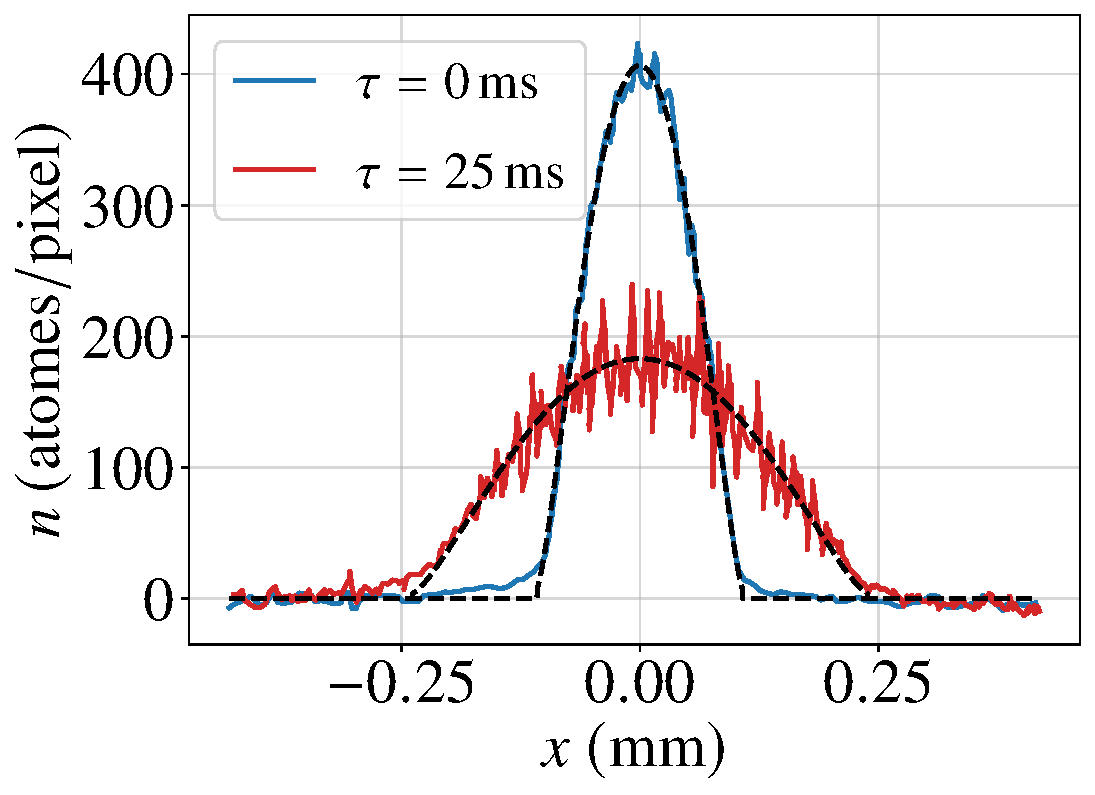
\includegraphics[width=0.45\textwidth]{./figures/05_Disp_Exp/fit_n_vs_tau.pdf}};
        	\node[above=-0.2cm of a , shift={(-2 , 0)}] {(a)};	
        \end{scope}

        
        
        % Deuxième figure
        \begin{scope}[shift={(7,0)}]
        	\node (b) at (0,0) {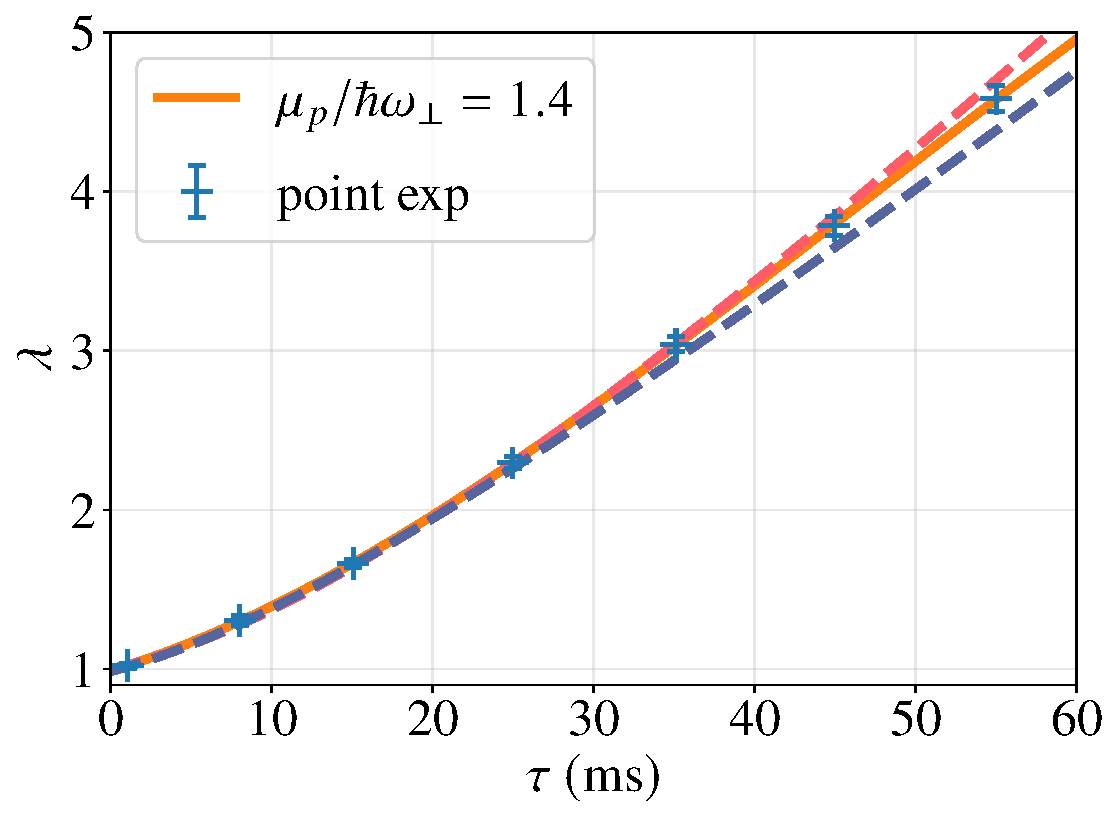
\includegraphics[width=0.45\textwidth]{./figures/05_Disp_Exp/fit_lambda_vs_tau.pdf}};
        	\node[above=-0.2cm of b , shift={(-2 , 0)}] {(b)};
        	
        	\draw[thick, color=colorSix, line width = 0.5ex , <-]
    			(1,1) to[out=180, in=90] (-2,-0.)
    			node[below, color = colorSix] { \color{\colorSix} \small TF 3D : $\mu_p \gg \hbar \omega_\perp$};	
    		\draw[thick, color=colorFour, line width = 0.5ex , <-]
    			(1.9,1) to[out=-90, in=90] (2,-0.5)
    			node[below, color = colorFour] { \color{\colorFour} \small TF 3D : $\mu_p \gg \hbar \omega_\perp$};	
        \end{scope}

        
	\end{tikzpicture}
	\caption{
(a) Profil de densité à l'équilibre dans le piège harmonique longitudinal (bleu), ajusté par $n_0(x)$ selon Eq.~\eqref{chap:eq:ajust} (noir pointillé). La courbe rouge montre le profil après une expansion longitudinale $\tau = 25~\mathrm{ms}$, avec un facteur d'échelle $\lambda$ extrait en ajustant le profil par une courbe homothétique à la densité initiale (noir pointillé), cf. Eq.~\eqref{chap:5:eq.hydro.1.3}.  
(b) Points bleus : facteurs d'échelle $\lambda(\tau)$ extraits expérimentalement. Courbe orange : résultats numériques obtenus en résolvant les équations hydrodynamiques (Eq.~\eqref{chap4:eq.pot.s.1}) avec $\mu_p / \hbar \omega_\perp = 1.4$. Les courbes pointillées montrent les évolutions attendues de $\lambda$ en résolvant Eq.~\eqref{chap:5:eq.hydro.3.4} pour $\alpha = 1$ (TF 1D) et $\alpha = 1/2$ (TF 3D).
}

	\label{fig:profil}
\end{figure}



% --- Table révisée (petites corrections typographiques) ---
%\begin{table}[h]
%\centering
%\begin{tabular}{l c c c}
%\hline
%Système & loi pour $\mu(n)$ & $\beta$ (avec $f(\lambda)=\lambda^{-\beta}$) & $\displaystyle \omega_{\rm breath}/\omega_\parallel$ \\
%\hline
%Gaz classique isotherme (1D, $\mu\propto\ln n$) 
%& $\mu'(n)\propto 1/n$ 
%& $-1$ 
%& $\sqrt{3}\approx1.732$ \\[4pt]
%
%Gaz de Bose 1D en régime moyen (GP, $\mu\propto n$) 
%& $\alpha=1$ 
%& $0$ 
%& $2$ \\[4pt]
%
%Tonks--Girardeau (1D, $\mu\propto n^2$) 
%& $\alpha=2$ 
%& $1$ 
%& $\sqrt{5}\approx2.236$ \\[4pt]
%
%Gaz de Fermi unitaire (ex. 3D, $\mu\propto n^{2/3}$) 
%& $\alpha=\tfrac{2}{3}$ 
%& $-\tfrac{1}{3}$ 
%& $\sqrt{3+\tfrac{2}{3}}\approx1.915$ \\[4pt]
%
%Cas général (loi de puissance) 
%& $\mu\propto n^\alpha$ 
%& $\beta=\alpha-1$ 
%& $\displaystyle \sqrt{3+\alpha}$ \\
%\hline
%\end{tabular}
%\caption{Valeurs de $\beta$ et fréquences du mode de souffle pour quelques régimes usuels.}
%\label{tab:breathing}
%\end{table}
% 



\subsection{Sonde locale de distribution de rapidité}


\subsubsection{Distribution de rapidités locale dans les gaz 1D}

%\paragraph{Motivation.}  
%La compréhension des gaz de bosons 1D avec interactions de contact répulsives repose sur la notion de distribution de rapidités \(\rho(\theta)\). Chaque état propre du système peut être paramétré par un ensemble de rapidités \(\{\theta_i\}\) , ou interprété comme les vitesses de quasi-particules à durée de vie infinie. Ici, on utilise la définition pratique issue des expansions 1D : les rapidités correspondent aux vitesses asymptotiques des atomes après une expansion, avec \(x_j \simeq \tau \theta_j\) pour un temps \(\tau\) long \footnote{Dans une article \cite{bezzaz2023rapiditydistributiondefocusingnonlinear} on voit que La limite champ classique du gaz de Lieb Liniger correspond à l’Équation de
%Schrödinger Non-Linéaire. Dans ce cadre, la théorie de diffusion inverse permet
%de construire un ensemble de quantités conservées.
%— Une méthode permettant de faire le lien entre la distribution de rapidité et
%les quantités conservées issues de la théorie de diffusion inverse est d’utiliser
%la définition de la distribution de rapidités comme distribution en impulsion
%asymptotique des atomes après une expansion 1D. On retrouve alors un résultat
%connu. J'ai bien cette aproche avec l'inverse scatering }. 
%\begin{eqnarray*}
%	\tilde{n}(v , \tau ) \underset{\tau \to \infty}{\rightarrow} \Pi (v).
%\end{eqnarray*}
%Cette définition est directement applicable à des mesures expérimentales de distribution de rapidités locales car à temps long la distribution spatial devient homotétique à la distribution de vitestes $\tau n (x , \tau ) \underset{\tau \to \infty}{\rightarrow} n (x/\tau , \tau) $ soit 
%\begin{eqnarray*}
%	\tau n (x , \tau )	 \underset{\tau \to \infty}{\rightarrow} \Pi (x/\tau).
%\end{eqnarray*}

\paragraph{Motivation.}  
La compréhension des gaz de bosons unidimensionnels avec interactions de contact répulsives repose sur la notion de distribution de rapidités \(\rho(\theta)\). Chaque état propre du système peut être caractérisé par un ensemble de rapidités \(\{\theta_i\}\), interprétées comme les vitesses de quasi-particules à durée de vie infinie.  

Dans le cadre des expansions 1D, une définition pratique consiste à assimiler les rapidités aux vitesses asymptotiques des atomes après une expansion libre, via la relation \(x_j \simeq \tau \theta_j\) pour un temps d’expansion long \(\tau\) \footnote{Dans la limite champ classique, le gaz de Lieb–Liniger est décrit par l’équation de Schrödinger non-linéaire. La théorie de diffusion inverse permet alors de construire un ensemble de quantités conservées. Dans ce cadre, la distribution de rapidités peut être définie comme la distribution en impulsion asymptotique des atomes après une expansion 1D, ce qui établit un lien direct entre rapidités et quantités conservées \cite{bezzaz2023rapiditydistributiondefocusingnonlinear}}.
.  

Ainsi, la distribution de vitesses mesurée à long temps tend vers la distribution de rapidités \(\Pi(v)\) :  
\[
	\tilde{n}(v , \tau ) \underset{\tau \to \infty}{\longrightarrow} \Pi(v).
\]  
Cette définition est directement exploitable expérimentalement : à temps long, la distribution spatiale devient homothétique à la distribution de vitesses,  
\[
	\tau n(x , \tau ) \underset{\tau \to \infty}{\longrightarrow} \Pi(x/\tau).
\] 


\paragraph{Distribution locale et LDA.}  
Pour un nuage atomique piégé dans un potentiel longitudinal variant lentement, on peut appliquer la \gls{LDA}. Le gaz est alors vu comme un fluide décomposé en cellules mésoscopiques de densité homogène et relaxée. Dans chaque cellule, l’état d’équilibre est décrit par un \gls{GGE}, ou équivalemment par une distribution de rapidités locale \(\rho(x,\theta)\). Cette description permet d’étudier non seulement l’équilibre, mais aussi la dynamique hors équilibre à grandes échelles spatiales et temporelles, via la théorie \gls{GHD}.

\paragraph{Protocole expérimental.}  
Pour mesurer \(\rho(x,\theta)\) localement :  
\begin{enumerate}
    \item Une zone du nuage atomique de taille \(\ell\) centrée en \(x_0\) est sélectionnée à l’aide du \gls{DMD}. La pression de radiation supprime instantanément les atomes en dehors de la zone, laissant uniquement ceux de la cellule (Fig ~\ref{fig:selection}).
    \item Après la sélection, le confinement longitudinal est relâché, tandis que le confinement transverse reste actif. Les atomes réalisent une expansion 1D pendant un temps \(\tau\), puis le profil de densité est imagé (typiquement pour \(\tau\sim 60\) ms).
    \item Le protocole est répété pour plusieurs positions \(x_0\), permettant d’obtenir la distribution de rapidités locale sur l’ensemble du nuage.
\end{enumerate}

\begin{figure}[H]
	\centering
	\begin{tikzpicture}
		%\begin{scope}[transform canvas={scale=0.6}]
	
		\begin{scope}[shift={(0,0)}]
			
		


        \begin{scope}[shift={(0,0)}, transform canvas={scale=0.5}]
        	\draw[thick, color = \colorFour , fill = \colorFour,line width = 0.5ex ] (0,0) ellipse [x radius=4cm, y radius=0.2cm];
        	\draw 
        		(-5 , 0 ) edge[thick, color=colorOne, line width = 0.5ex , ->] node[pos = 1.0 ,   below , color = \colorOne]{\fontsize{18}{20}\selectfont  $x$}  (5,0)
        		(0,-1) edge[thick, color=colorOne, line width = 0.5ex , ->] node[pos = 1.0 , left , color = \colorOne]{\fontsize{18}{20}\selectfont  $y$} (0,1)
        		
        		(1,-0.3) edge[thick, color=colorThree, line width = 0.4ex ] node[pos = 0.0 , below , color = \colorThree]{\fontsize{18}{20}\selectfont  $x_0$} (1,0.3)
        		
        		(-0.5,0) edge[shift = {(1,0.45)} , thick, color=colorThree, line width = 0.4ex , <->] node[pos = 0.5 , above , color = \colorThree]{\fontsize{18}{20}\selectfont  $\ell$} (0.5,0)
        		
        		(0,0) edge[shift = {(-3,0.5)} , thick, color=colorOne, line width = 0.4ex , <-] node[shift = {(0,-0.1)} , pos = 1 , above , color = \colorOne]{\fontsize{15}{20}\selectfont  $5\, \mu m $} (0,0.25)
        		(0,0) edge[shift = {(-3,-0.5)} , thick, color=colorOne, line width = 0.4ex , <-] (0,-0.25)
        	;
        	 % Contour
			\draw[line width=0.4ex, color=colorSix]
    			(1.5,-0.5) rectangle +(3,1)
    			(0.5,-0.5) rectangle +(-5,1);

			% Remplissage avec hachures épaisses
			\fill[pattern={Lines[angle=-45,distance={5pt},line width=0.4ex]}, pattern color=colorSix]
    			(1.5,-0.5) rectangle +(3,1)
    			(0.5,-0.5) rectangle +(-5,1);
    		
    		\draw[thick, color=colorSix, line width=0.5ex, <-]
    			(-2,-0.4) to[out=-90, in=0] (-2.4,-1.3)
   				 node[left, color=colorSix, align=left] 
    			{\fontsize{12pt}{14pt}\selectfont \bfseries \itshape
    			faisceau lumineux\\
    			\bfseries \itshape façonné par le DMD}
    		;
    		\draw[thick, color=colorFour, line width=0.5ex, <-]
    			(-1,-0.0) to[out=-90, in=-180] (1,-1.3)
   				 node[right, color=colorFour, align=left] 
    			{\fontsize{12pt}{14pt}\selectfont \bfseries \itshape
    			nuage atomique}
    		;	
        		
        \end{scope}
        \draw [color = white] (-3,-1) rectangle +(10,2);
		\node[shift={(-3 , 1)}] at (0,0) {a)};
     	\end{scope}
     	
     	 % Deuxième figure
        \begin{scope}[shift={(7,0)}]
        	\node (b) at (0,0) {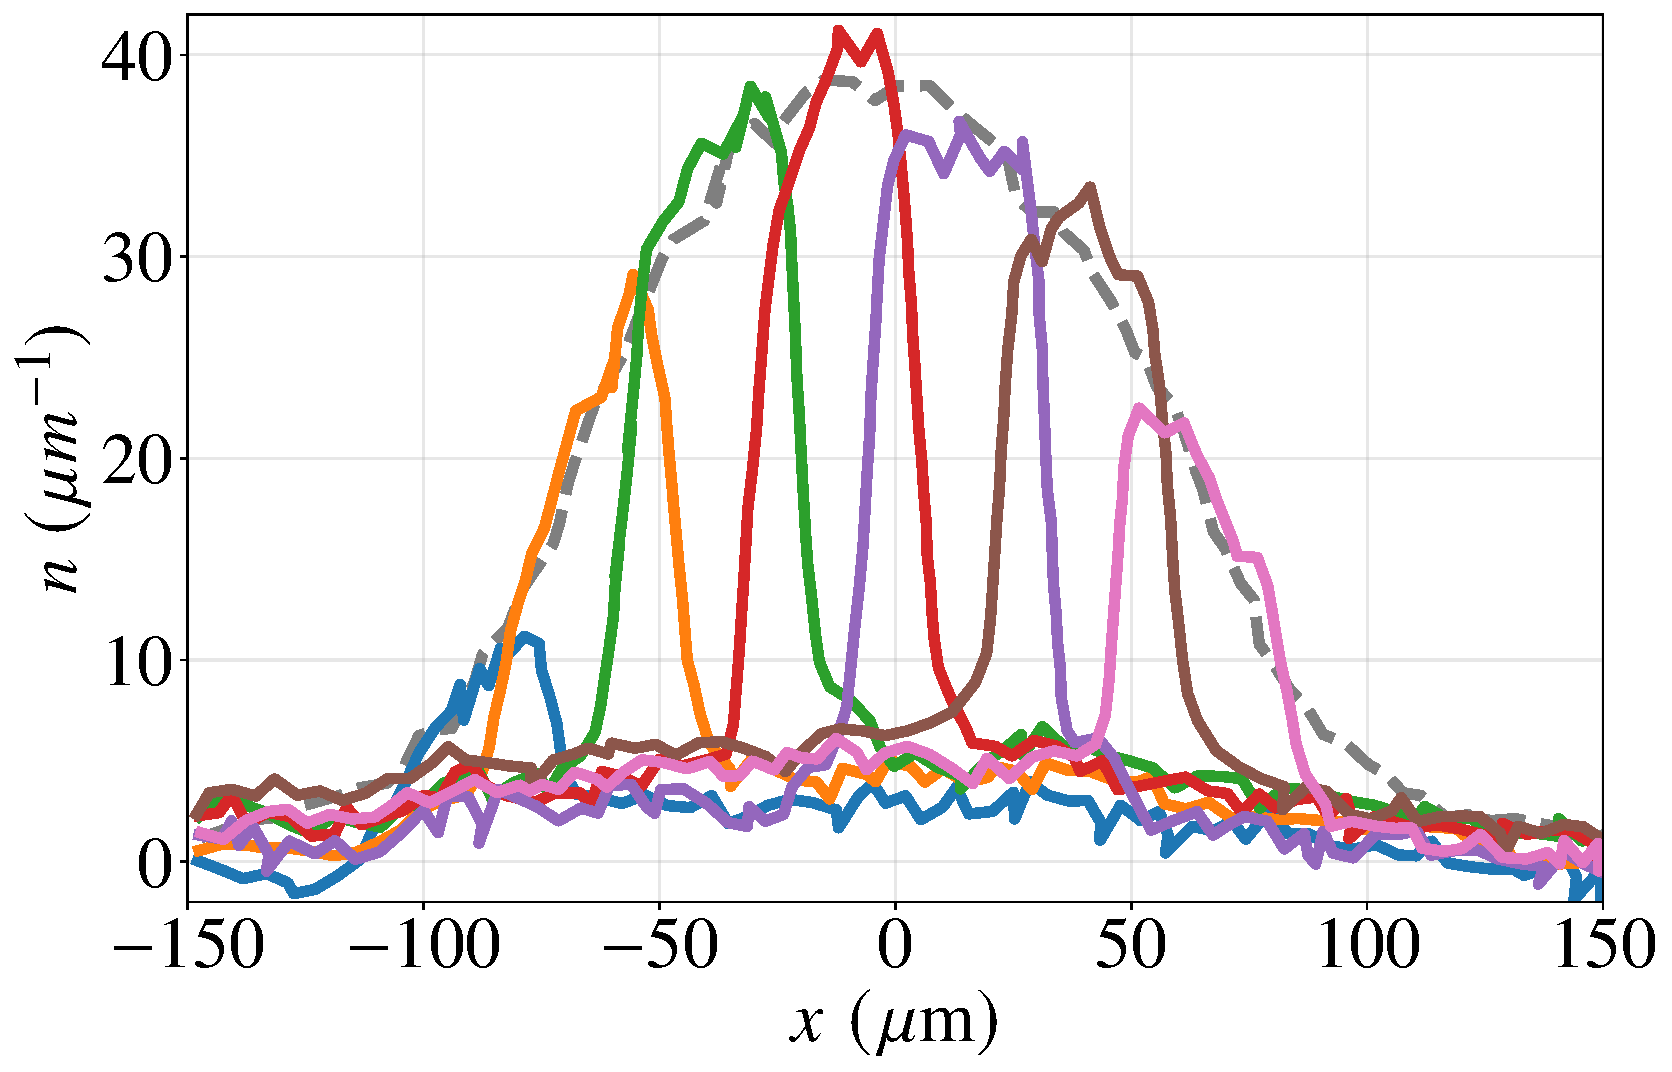
\includegraphics[width=0.55\textwidth]{./figures/05_Disp_Exp/profils.pdf}};
        	\node[above=-0.2cm of b , shift={(-2 , 0)}] {b)};
        	
%        	\draw[thick, color=colorSix, line width = 0.5ex , <-]
%    			(1,1) to[out=180, in=90] (-2,-0.)
%    			node[below, color = colorSix] { \color{\colorSix} \small TF 3D : $\mu_p \gg \hbar \omega_\perp$};	
%    		\draw[thick, color=colorFour, line width = 0.5ex , <-]
%    			(1.9,1) to[out=-90, in=90] (2,-0.5)
%    			node[below, color = colorFour] { \color{\colorFour} \small TF 3D : $\mu_p \gg \hbar \omega_\perp$};	
        \end{scope}

        
	\end{tikzpicture}
	\caption{(a) Schéma illustrant la sélection d’une région du nuage atomique, ici représentée par un ellipse bleu illuminé par un faisceau modulé à l’aide du DMD.\\
(b) Exemple de sélections sur un gaz initialement à l’équilibre : superposition du profil de densité initial du nuage (courbe grise) et des profils mesurés après $\tau = 1~\mathrm{ms}$ pour différentes régions de sélection de taille $\ell = 37~\mu\mathrm{m}$ centrées en différentes positions $x_0$ (courbes colorées).
}

	\label{fig:selection}
\end{figure}

\paragraph{Mesures à l’équilibre.}  
Pour un gaz initialement à l’équilibre dans un piège harmonique, le profil de densité de chaque zone sélectionnée est analysé via \gls{TBA} et la \gls{LDA}, donnant température \(T\) et potentiel chimique \(\mu\). Après un temps d’expansion long, le profil devient homothétique à la distribution de rapidités locale \(\rho(x,\theta)\). La comparaison avec les prédictions numériques montre une bonne cohérence, confirmant que le protocole permet de sonder efficacement \(\rho(x,\theta)\).


\begin{figure}[H]
	\centering
	\begin{tikzpicture}
		%\begin{scope}[transform canvas={scale=0.6}]
	
		\begin{scope}[shift={(0,0)}]
			
			\node (a) at (0,0) {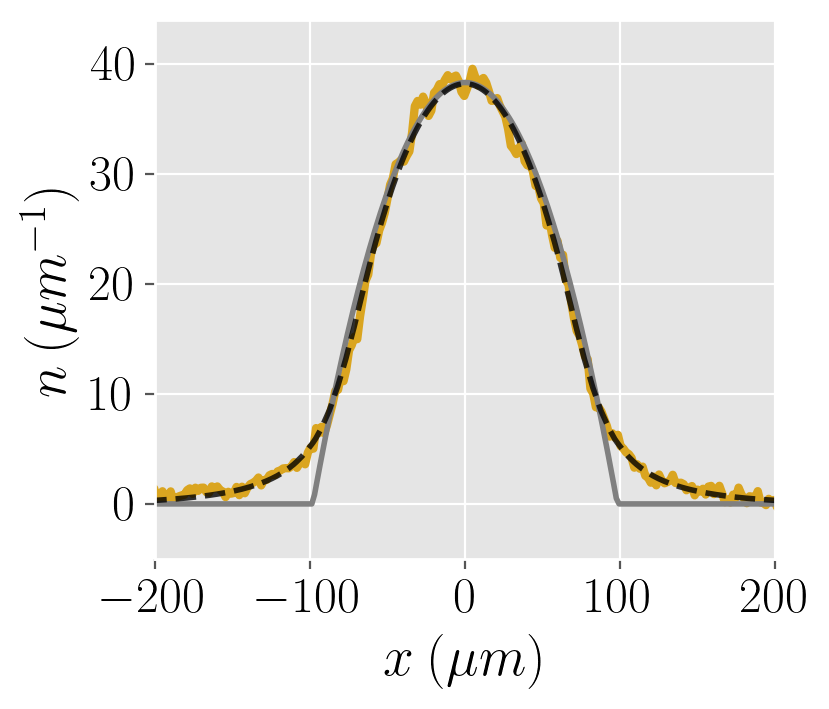
\includegraphics[width=0.3\textwidth]{./figures/05_Disp_Exp/image159.png}};
        	\node[above=-0.2cm of a , shift={(-2 , 0)}] {a)};


                
        %\draw [color = white] (-3,-1) rectangle +(10,2);

     	\end{scope}
     	
     	 % Deuxième figure
        \begin{scope}[shift={(7,0)}]
        	\node (b) at (0,0) {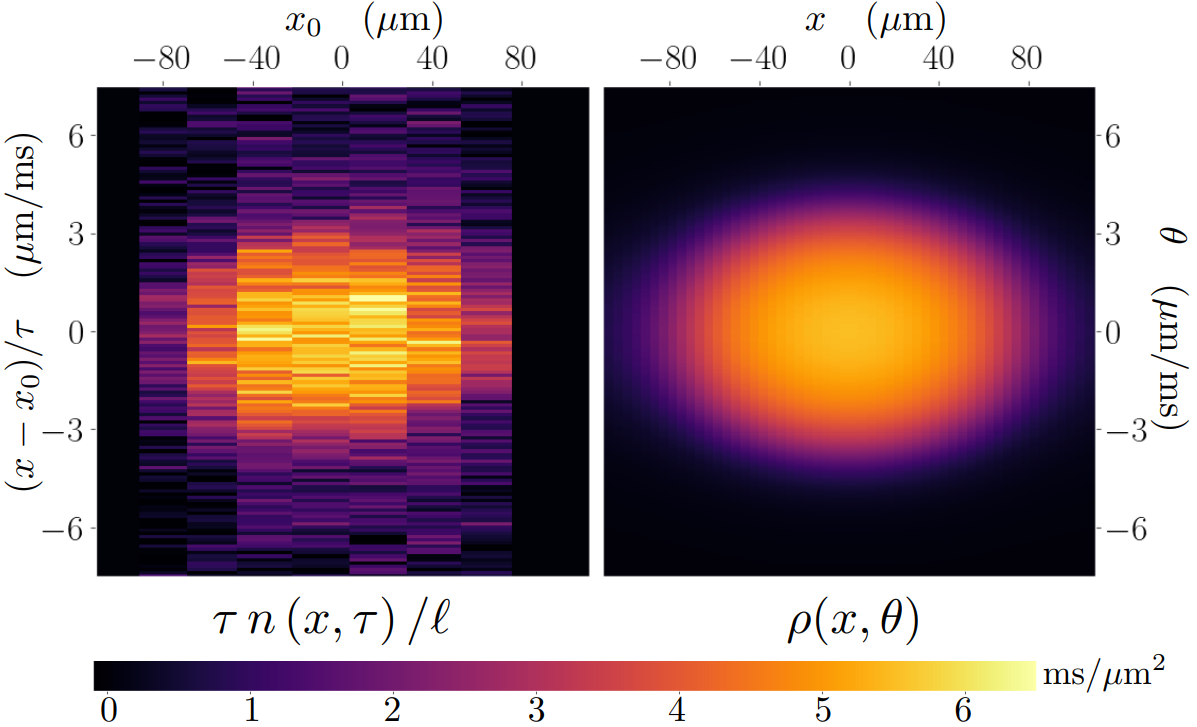
\includegraphics[width=0.6\textwidth]{./figures/05_Disp_Exp/image212.png}};
        	\node[above=-0.2cm of b , shift={(-3.2 , -1.3)} , color = white ] {\color{white} b1)};
        	\node[above=-0.2cm of b , shift={(0.5 , -1.3)} , color = white ] {\color{white} b2)};
        	
        \end{scope}

        
	\end{tikzpicture}
	\caption{a) Profil de densité d’un nuage atomique initialement à l’équilibre dans un piège harmonique avec $\omega_\perp = 2 \pi \times  2.6~\mathrm{kHz}$ et $\omega_\parallel = 2 \pi \times 5~\mathrm{Hz}$ (zone en jaune). La courbe grise représente le profil parabolique attendu à l’état fondamental dans le régime qBEC, décrit par l’équation d’état $n(x) = [\mu - V_\parallel(x)]/g$. La courbe noire en pointillés correspond à un ajustement des données expérimentales en supposant que le système soit bien décrit par un ensemble thermique (\gls{TBA} (Sec ~ \ref{chap4:sec:TBA})). Cet ajustement permet d’extraire une température $T = 90~\mathrm{nK}$ et un potentiel chimique $\mu/k_B = 49~\mathrm{nK}$.
	(b1) Profils de densités pour différents centres de sélection x0 représentés sur la Fig.\ref{fig:selection}(b). Les sélections sont de taille $\ell = 37\, \mu m$ et les profils obtenus après un temps d’expansion $\tau =  40 \, ms$. Pour comparer les résultats à une distribution de rapidités, les profils de densités sont multipliés par le rapport $\tau/ \ell$ et sont tracés en fonction de $(x-x_0)/\tau$ (b2). (b2) Prédiction théorique de la distribution de rapidités spatialement résolue $\rho ( x , \theta)$ à l’équilibre thermique dans un potentiel harmonique longitudinal avec $\omega_\parallel = 2 \pi \times 5~\mathrm{Hz}$. La température $T$ et le potentiel chimique $\mu$ utilisés sont eux obtenus à partir du profil in situ (a).}
	\label{fig:expansion}
\end{figure}

\paragraph{Résumé.}  
— Une sonde locale de distribution de rapidités a été mise en place grâce au \gls{DMD}.  
— Les atomes sélectionnés réalisent une expansion dans le guide 1D.  
— Après un temps long, le profil de densité reflète la distribution de rapidités locale.  
— Ce protocole a été appliqué avec succès sur un nuage atomique initialement à l’équilibre.

\paragraph{Dynamique.}
\subparagraph{Motivation.}
Pour vérifier si le régime asymptotique des expansions longitudinales est atteint, il est nécessaire de comparer les résultats expérimentaux à une théorie dynamique. L’outil adapté est de \gls{GHD}, déjà introduite au Chapitre~\ref{chap:GHD}, qui décrit l’évolution spatio-temporelle de la distribution de rapidités.

\subparagraph{Invariance d’échelle hydrodynamique.}
On considère une sélection initiale homogène de taille $\ell$ centrée en $x_0$. Dans ce cas, les équations \gls{GHD} \eqref{chap:GHD:eq.conserv.3.1} s’écrivent sans potentiel, avec la condition initiale $\rho(x,\theta,0)=\rho_0(\theta)$ si $|x-x_0|\leq \ell/2$, et $0$ sinon. En introduisant les variables sans dimension $\alpha=(x-x_0)/\ell$ et $\beta=\tau/\ell$, l’équation devient indépendante de $\ell$. 
\begin{eqnarray*}
	\left \{ 
	\begin{array}{rcl}
		\partial_\beta \tilde{\rho} ( \alpha , \theta ; \beta ) +  \partial_x ( v^{\mathrm{ell}}_{[\tilde{\rho}]} (\theta)  \tilde{\rho} ( \alpha , \theta ; \beta )) = 0 \\
		\tilde{\rho} ( \alpha , \theta ; 0 )	 = \begin{cases}
			\rho_0(\theta) & \text{si } |\alpha|\leq \tfrac{1}{2}, \\
			0 & \text{sinon},
		\end{cases}% \rho_0(\theta) \, \mbox{si} \, \vert \alpha \vert \leq \frac12 \,, \,  0 \, \mbox{sinon}.
	\end{array}
	\right .
\end{eqnarray*}
Il en résulte que les profils de densité $n(x,\tau)$, exprimés en fonction de $\alpha$, ne dépendent que du rapport $\beta$. 
Autrement dit, deux sélections de tailles différentes mais telles que $\tau/\ell$ soit constant doivent conduire aux mêmes profils après expansion. Cette invariance a été vérifiée expérimentalement : les profils se superposent de manière remarquable (Fig ~\ref{fig:scail2} a)) .

\subparagraph{Lien avec les équations de Gross–Pitaevskii}
Dans le régime \gls{qBEC}, à basse température, la dynamique peut aussi être décrite par les équations hydrodynamiques issues de \gls{GP} (en négligeant la pression quantique) 
Après changement de variables ($\alpha=(x-x_0)/\ell$, $\beta=\tau/\ell$, $\tilde n=n/n_0$), on retrouve un système d’équations qui ne dépend plus de $\ell$, mais uniquement du rapport adimensionné $\eta=\beta g n_0/m$.
\begin{eqnarray*}
	\left \{ 
	\begin{array}{rcl}
		\partial_\beta \tilde n + \partial_\alpha ( \tilde v \tilde n) = 0, && \partial_\beta \tilde v + \tilde v \,\partial_\alpha \tilde v = - \dfrac{g n_0}{m}\,\partial_\alpha \tilde n, \\[6pt]
	\tilde n(\alpha,\beta=0) = 
		\begin{cases}
			1 & \text{si } |\alpha|\leq \tfrac{1}{2}, \\
			0 & \text{sinon},
		\end{cases}, && 
\tilde v(\alpha,\beta=0)=0.
	\end{array}
	\right.
\end{eqnarray*}
Il en découle que les profils de densité sont universels lorsqu’ils sont exprimés en fonction de $(\alpha,\eta)$. Expérimentalement, ce comportement est bien confirmé : les centres des profils se superposent pour des conditions initiales différentes, et l’accord est même bon sur les bords (Fig ~\ref{fig:scail2} b)) .

\begin{figure}[H]
	\centering
	\begin{tikzpicture}
		%\begin{scope}[transform canvas={scale=0.6}]
	
		\begin{scope}[shift={(0,0)}]
			
			\node (a) at (0,0) {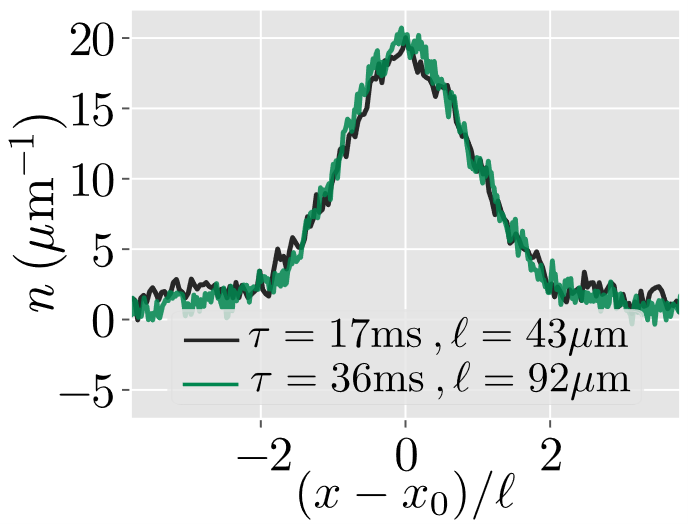
\includegraphics[width=0.5\textwidth]{./figures/05_Disp_Exp/image246.png}};
        	\node[above=-0.2cm of a , shift={(-2 , -1)}] {\color{black} a)};


                
        %\draw [color = white] (-3,-1) rectangle +(10,2);

     	\end{scope}
     	
     	 % Deuxième figure
        \begin{scope}[shift={(7,0)}]
        	\node (b) at (0,0) {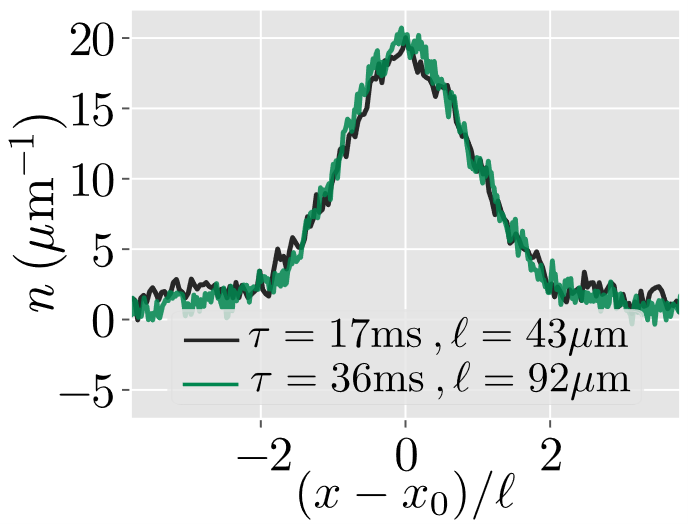
\includegraphics[width=0.5\textwidth]{./figures/05_Disp_Exp/image246.png}};
        	\node[above=-0.2cm of b , shift={(-2 , -1.)} ] {\color{black} b)};
        	
        	
        \end{scope}

        
	\end{tikzpicture}
	\caption{(a) Illustration du comportement hydrodynamique prédit par les équations de GHD. Deux profils de densité sont représentés en fonction de $\alpha$ pour un même paramètre $\beta = \tau / \ell = 0.39~\mathrm{ms}/\mu\mathrm{m}$.(b) Analyse du comportement hydrodynamique selon le formalisme GP. Deux profils de densité sont tracés pour un même ratio $\eta = (\tau/\ell)\, g n_0 / m = 2.65$, avec une taille de sélection $\ell = 37~\mu\mathrm{m}$, mais pour des densités initiales $n_0$ différentes. Les sélections ont été réalisées sur plusieurs régions distinctes d’un même nuage.
	}

	\label{fig:scail2}
\end{figure}

\subparagraph{Régime asymptotique.}  
L’expansion des tranches est bien décrite par \gls{GHD}. Les comparaisons entre données expérimentales et simulations \gls{GHD} (avec des distributions thermiques initiales) montrent un bon accord au centre des profils, mais révèlent que le régime asymptotique complet n’est pas atteint dans les temps accessibles expérimentalement. On définie un écart-type $$\sigma(\tau) = \sqrt{ \frac{\int \vert \frac{\tau}{\ell} n_{\mathrm{GHD}}( \frac{x-x_0}\tau) - \rho(\frac{x-x_0}\tau) \vert^2 d \tau }{ \int \vert \rho( \frac{x-x_0}\tau) \vert^2 d \tau} }$$ avec $n_{\mathrm{GHD}}$ les profil tirés des simulations \gls*{GHD}.Pour $\tau=50$\,ms, l’écart-type reste d’environ $12\%$, et une convergence complète nécessiterait des temps irréalistes ($\sim 500$\,ms). L’extraction de la distribution de rapidité à partir des profils reste donc approximative.

\begin{figure}[H]
	\centering
	\begin{tikzpicture}
		%\begin{scope}[transform canvas={scale=0.6}]
	
		\begin{scope}[shift={(0,0)}]
			
			\node (a) at (0,0) {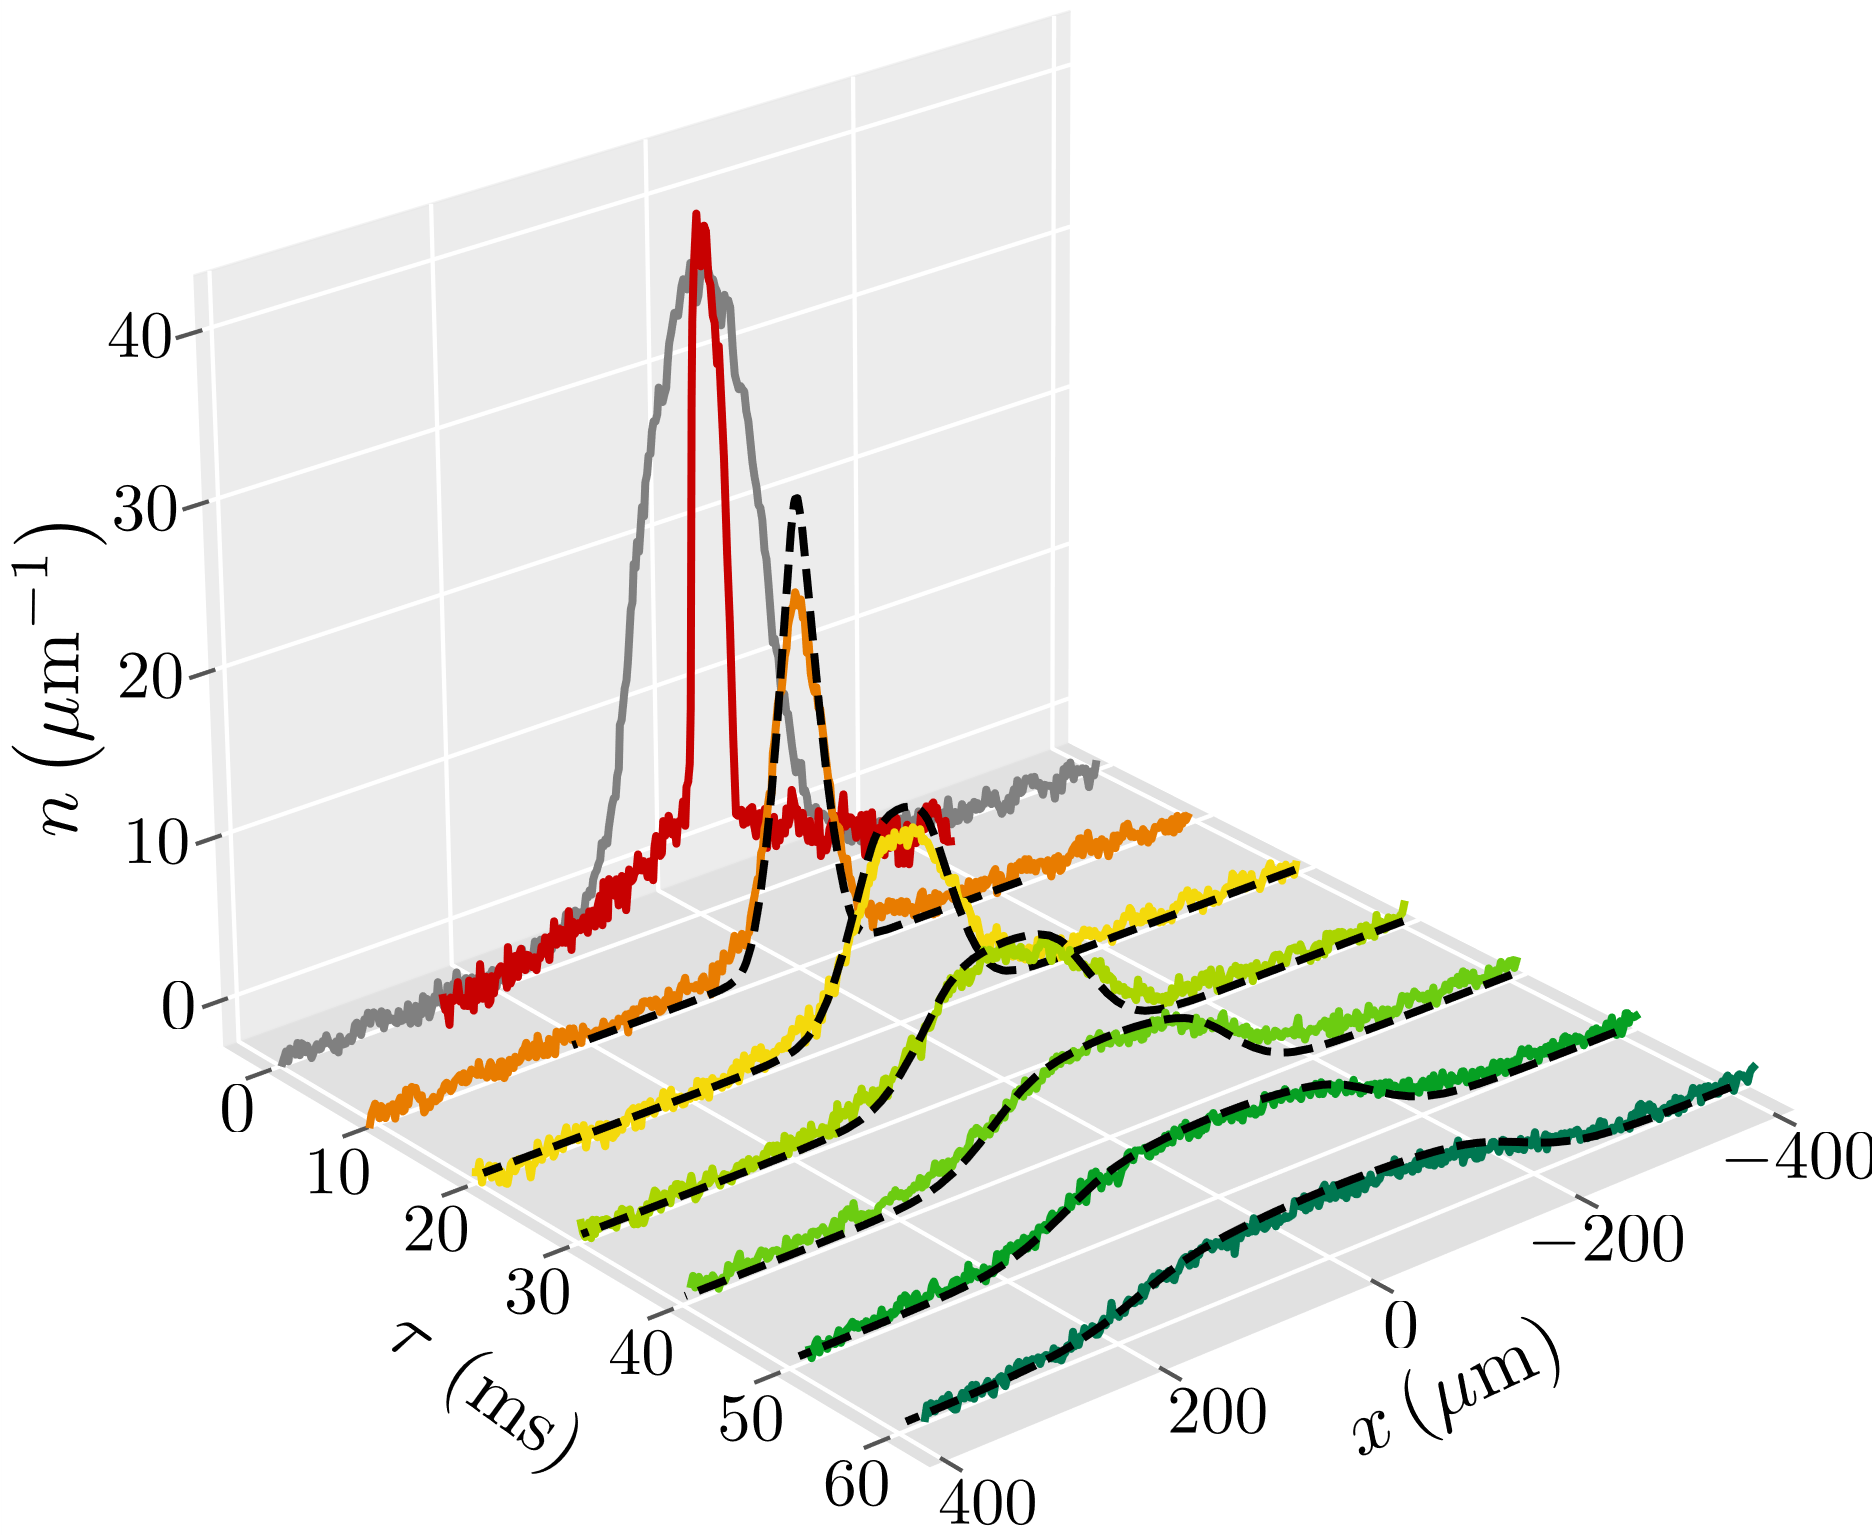
\includegraphics[width=0.7\textwidth]{./figures/05_Disp_Exp/image255.png}};
        	\node[above=-0.2cm of a , shift={(-2 , -1)}] {\color{black} a)};


                
        %\draw [color = white] (-3,-1) rectangle +(10,2);

     	\end{scope}
     	
     	 % Deuxième figure
        \begin{scope}[shift={(7,0)}]
        	\node (b) at (0,0) {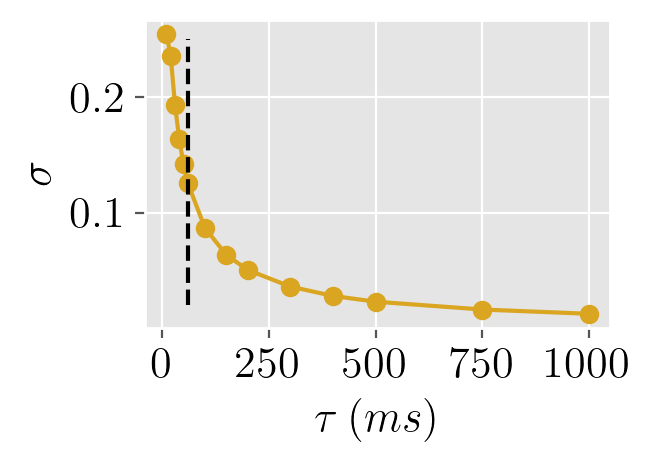
\includegraphics[width=0.3\textwidth]{./figures/05_Disp_Exp/image265.png}};
        	\node[above=-0.2cm of b , shift={(-2 , -1.)} ] {\color{black} b)};
        	
        	
        \end{scope}

        
	\end{tikzpicture}
	\caption{(a) La tranche , centrée en $x_0 = 0\,\mu\mathrm{m}$ ,subit une expansion le long de l'axe longitudinalet d'une largeur $\ell = 37\,\mu\mathrm{m}$. Le profil initial du gaz est montré en gris. Les variations de densité pour différents temps d'expansion sont représentées par des courbes colorées. Les lignes pointillées noires indiquent les résultats des simulations GHD pour une distribution de rapidités initialement thermique, paramétrée par la température $T$ et le potentiel chimique $\mu(x_0)  = \mu$, tels qu'ils sont extraits du profil de densité in situ.(b) L'écart-type $\sigma(\tau) = \sqrt{ \int \vert \frac{\tau}{\ell} n _{\mathrm{GHD}}( (x-x_0)/\tau) - \rho( (x-x_0)/\tau) \vert^2 d \tau / \int \vert \rho( (x-x_0)/\tau) \vert^2 d \tau } $ défini par l'équation~(8.8) est calculé entre la distribution de rapidités et les résultats des simulations GHD en fonction du temps d'expansion $\tau$. La ligne verticale noire correspond au temps d'expansion utilisé dans l'expérience.
}

	\label{fig:GHD1}
\end{figure}

%\subparagraph{Hypothèse thermique.}  
%Afin de restreindre le nombre de paramètres d’ajustement, on suppose que la distribution de rapidité locale est thermique. Dans ce cas, seule la température $T$ est ajustée, le potentiel chimique étant fixé par l’équation d’état. L’ajustement sur les profils expérimentaux conduit à une température effective $T_{\text{fit}}=230$\,nK, environ 2.5 fois plus grande que celle extraite à l’équilibre. Néanmoins, les distributions de rapidité obtenues restent proches, confirmant que, dans le régime fortement \gls{qBEC}, la dynamique dépend surtout des interactions et peu de la température. L’influence possible d’une faible population transversale excitée a été évaluée et s’est révélée négligeable.

\subsection*{8.6 Mesure locale de distribution de rapidités hors équilibre}

\paragraph{Mise en place d’une distribution locale hors équilibre.}  
Le faisceau de sélection (\gls{DMD}) permet non seulement de sonder la distribution de rapidités locale, mais aussi de créer des situations hors équilibre. Un protocole illustratif consiste à retirer les atomes d’une région centrale de taille $\ell_0 = 70\,\mu$m, puis à laisser le gaz évoluer librement longidutalement (1D). Après un temps $\tau = 15$\,ms, la distribution de rapidités développe une structure doublement piquée, très différente d’une distribution thermique. Une seconde sélection locale ($\ell=35\,\mu$m) suivie d’une expansion révèle expérimentalement ce profil, en excellent accord avec les simulations GHD (Fif ~\ref{fig:GHD2}).

\begin{figure}[H]
	\centering
	\begin{tikzpicture}
		%\begin{scope}[transform canvas={scale=0.6}]
	
		\begin{scope}[shift={(0,0)}]
			
			\node (a) at (0,0) {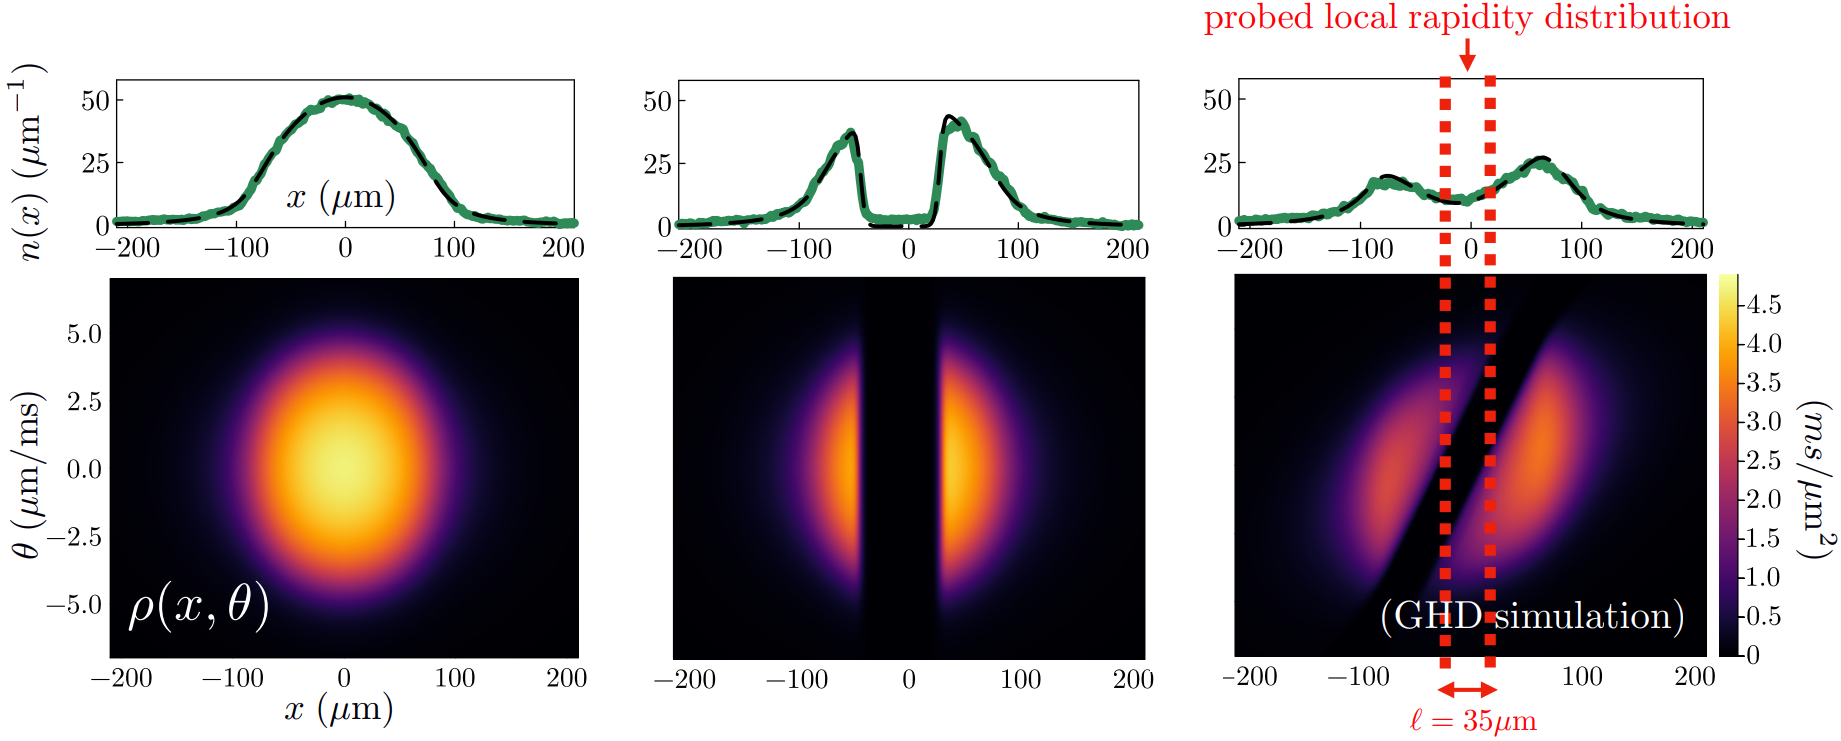
\includegraphics[width=0.6\textwidth]{./figures/05_Disp_Exp/image295.png}};
        	\node[above=-0.2cm of a , shift={(-2 , -1)}] {\color{black} a)};


                
        %\draw [color = white] (-3,-1) rectangle +(10,2);

     	\end{scope}
     	
     	 % Deuxième figure
        \begin{scope}[shift={(7,0)}]
        	\node (b) at (0,0) {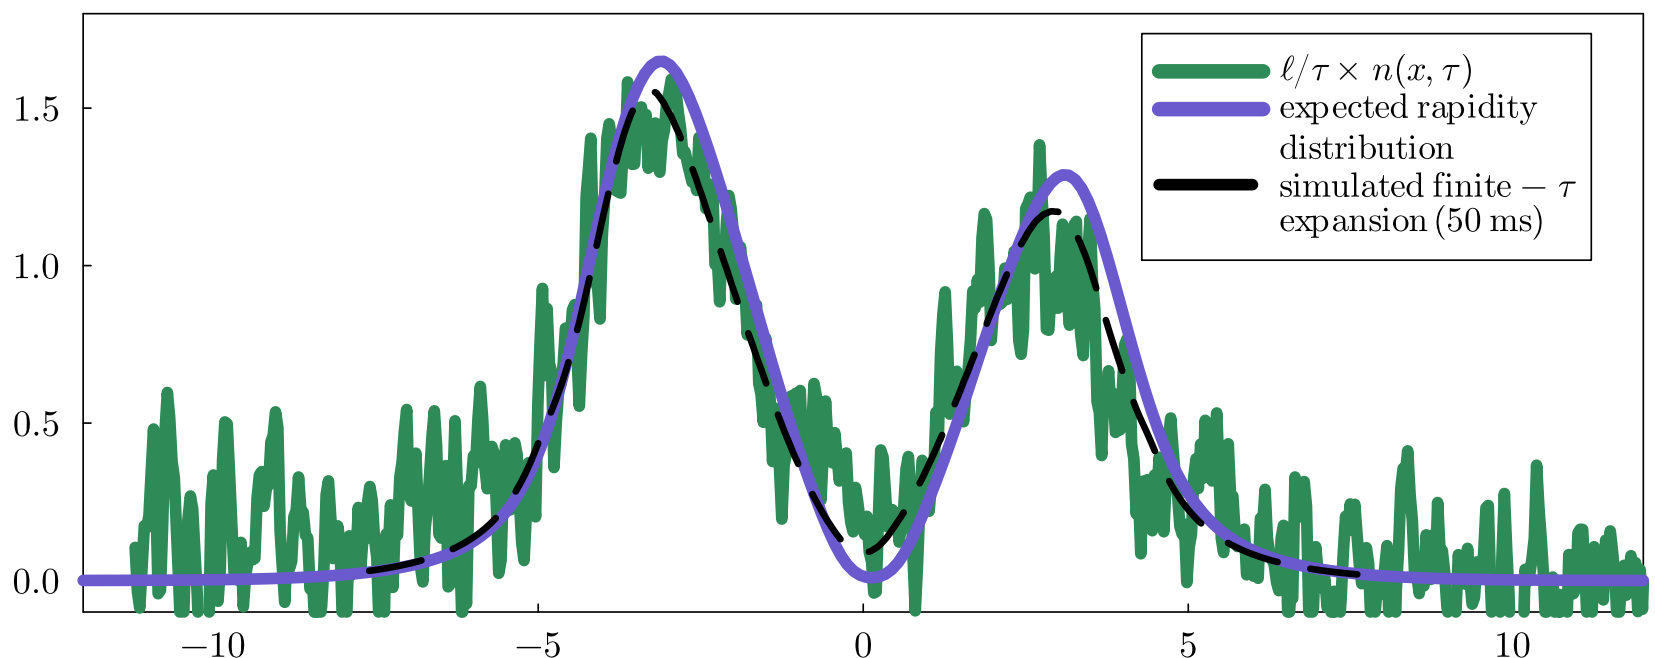
\includegraphics[width=0.4\textwidth]{./figures/05_Disp_Exp/image290.png}};
        	\node[above=-0.2cm of b , shift={(-2 , -1.)} ] {\color{black} b)};
        	
        	
        \end{scope}

        
	\end{tikzpicture}
	\caption{Les profils de densité sont montrés à différents stades : à l'équilibre initial (a1), 1\,ms après la première sélection (a2), et 15\,ms après une expansion le long du guide 1D (a3). Les distributions de rapidités résolues spatialement correspondantes sont illustrées dans les panels (a4) à (a6). Les lignes pointillées rouges indiquent la deuxième sélection.  (b)Pour obtenir la distribution locale de rapidités, on trace $\tau\, n(x,\tau)/\ell$ sur une région de largeur $\ell = 36\,\mu\mathrm{m}$ après un temps d'expansion longitudinal $\tau = 50\,\mathrm{ms}$. Le profil présente une double crête et montre un excellent accord avec la prédiction théorique de la distribution de rapidités (courbe violette), y compris les corrections dues à un temps d'expansion fini (courbe noire pointillée).
}

	\label{fig:GHD2}
\end{figure}

\paragraph{Analyse des distributions locales hors équilibre}  
Cette approche démontre l’importance d’une mesure locale : alors que la distribution globale $\int dx\,\rho(x,\theta)$ est conservée, la distribution locale $\rho(x,\theta)$ reflète directement la dynamique hors équilibre. Le dispositif basé sur le \gls{DMD} offre ainsi un outil puissant pour générer et caractériser divers protocoles hors équilibre (cisaillement, jonctions de densité, états stationnaires non thermiques, etc.), ouvrant de nouvelles perspectives pour l’étude des gaz de Bose 1D.


%\section{Discussion sur les limites et les perspectives}
%\begin{itemize}
%    \item Contraintes techniques (bruit, alignement, stabilité de la puce…).
%    \item Améliorations potentielles (résolution, contrôle du potentiel, automatisation).
%    \item Perspectives pour d’autres types d’expériences (étude de chocs, turbulence quantique, etc.)
%\end{itemize}
%
%\section*{Conclusion}
%\begin{itemize}
%    \item Résumé de l’architecture du dispositif).
%    \item Méthodes d’analyse utilisées et robustesse.
%    \item Importance de l’expérience dans le contexte de l’étude des gaz quantiques unidimensionnels
%\end{itemize}
%Ce chapitre a présenté les éléments essentiels du dispositif expérimental, les méthodes d’imagerie, ainsi que les expériences auxquelles j’ai participé. L’ensemble constitue une plateforme performante pour l’étude de la dynamique de gaz 1D hors équilibre.
%
%\paragraph{Résumé de l’architecture expérimentale}  
%Nous avons décrit les éléments clés du dispositif utilisé : un système de refroidissement laser basé sur trois sources couplées, un piégeage magnétique sur puce optimisé pour réaliser des géométries unidimensionnelles, une plateforme de modulation de potentiel via un DMD, et un système d’imagerie haute résolution. L’ensemble permet une manipulation fine des nuages atomiques dans un cadre reproductible et stable.
%
%\paragraph{Méthodes d’analyse et robustesse}  
%L’imagerie par absorption, couplée à une analyse rigoureuse des profils atomiques, fournit des outils fiables pour extraire les grandeurs pertinentes : densités, tailles, températures, distributions de vitesses. Ces méthodes ont permis de confronter les résultats expérimentaux à des prédictions théoriques de type GHD ou Yang-Yang.
%
%\paragraph{Importance du dispositif pour la thèse}  
%Ce dispositif a été essentiel pour mener à bien les expériences présentées dans cette thèse. Il offre à la fois un contrôle local (grâce au DMD), un bon confinement transverse (grâce à la puce) et une imagerie précise. La plateforme est ainsi bien adaptée pour étudier des systèmes 1D fortement corrélés hors équilibre, et pour tester les prédictions de la physique statistique intégrable.
%
%\paragraph{Perspectives}  
%Malgré ses atouts, le dispositif présente des limitations techniques (rugosité magnétique, sensibilité à l’alignement, etc.) qui laissent entrevoir des pistes d’amélioration. Des développements futurs pourraient notamment viser à augmenter la résolution spatiale, automatiser davantage les séquences, ou explorer d'autres régimes dynamiques comme la turbulence ou les collisions de chocs quantiques.
%
%
%
%%\appendix
%\section*{Annexes}
%\begin{itemize}
%    \item Schémas techniques (puce, DMD, optique).
%    \item Tableaux de paramètres expérimentaux.
%    \item Exemples de motifs DMD utilisés.
%\end{itemize}